\documentclass[12pt,a4paper]{report}

\usepackage[margin=1in,headheight=22pt,headsep=0.28in]{geometry}
\usepackage[T1]{fontenc}
\usepackage{helvet}
\renewcommand{\familydefault}{\sfdefault}
\usepackage{setspace}
\setstretch{1.15}
\usepackage{graphicx}
\usepackage{booktabs}
\usepackage{longtable}
\usepackage{array}
\usepackage{tabularx}
\usepackage[table]{xcolor}
\usepackage{hyperref}
\usepackage{listings}
\usepackage{enumitem}
\usepackage{float}
\usepackage{caption}
\usepackage{amsmath}
\usepackage{amssymb}
\usepackage{pgfplots}
\usepackage{needspace}
\usepackage{fancyhdr}
\usepackage{titlesec}
\usepackage{chngcntr}
\usepackage{tocloft}
\usepackage{etoolbox}
\pgfplotsset{compat=1.18}

\definecolor{covergreen}{RGB}{35,107,72}
\definecolor{accentgreen}{RGB}{224,239,228}
\definecolor{warningyellow}{RGB}{252,244,210}

\hypersetup{
  colorlinks=true,
  linkcolor=black,
  urlcolor=black,
  citecolor=black,
  plainpages=false,
  hypertexnames=false
}

\titleformat{\chapter}[hang]
  {\normalfont\bfseries\fontsize{24}{29}\selectfont\raggedright}
  {\chaptername\ \thechapter:}{0.5em}{}
\titleformat{name=\chapter,numberless}[hang]
  {\normalfont\bfseries\fontsize{24}{29}\selectfont}{}{0pt}{}
\titlespacing*{\chapter}{0pt}{0pt}{18pt}
\titleformat{\section}
  {\normalfont\bfseries\fontsize{18}{22}\selectfont}
  {\thesection}{0.6em}{}
\titlespacing*{\section}{0pt}{17pt}{8pt}
\titleformat{\subsection}
  {\normalfont\bfseries\fontsize{14}{18}\selectfont}
  {\thesubsection}{0.6em}{}
\titlespacing*{\subsection}{0pt}{13pt}{6pt}
\titleformat{\subsubsection}
  {\normalfont\bfseries\fontsize{12}{15}\selectfont}
  {\thesubsubsection}{0.6em}{}

\pagestyle{fancy}
\fancyhf{}
\fancyhead[R]{\textbf{Accelera} \textcolor{covergreen}{2026}}
\fancyfoot[R]{\thepage\,|\,Page}
\renewcommand{\headrulewidth}{0.5pt}
\renewcommand{\footrulewidth}{0.3pt}
\fancypagestyle{plain}{\pagestyle{fancy}}

\counterwithin{figure}{chapter}
\counterwithin{table}{chapter}
\renewcommand{\lstlistingname}{Algorithm}
\renewcommand{\lstlistlistingname}{List of Algorithms}

\lstdefinestyle{code}{
  basicstyle=\ttfamily\footnotesize,
  breaklines=true,
  frame=single,
  columns=fullflexible,
  keepspaces=true,
  showstringspaces=false,
  keywordstyle=\color{blue!60!black},
  commentstyle=\color{green!40!black},
  stringstyle=\color{red!50!black}
}

\lstdefinestyle{algostyle}{
  basicstyle=\ttfamily\footnotesize,
  backgroundcolor=\color{white},
  frame=tb,
  rulecolor=\color{black},
  framerule=0.45pt,
  framesep=4pt,
  columns=fullflexible,
  keepspaces=true,
  showstringspaces=false,
  breaklines=true,
  breakatwhitespace=false,
  breakautoindent=false,
  breakindent=0pt,
  captionpos=t,
  aboveskip=0.8em,
  belowskip=0.8em
}

\setlength{\emergencystretch}{2em}
\raggedbottom
\renewcommand{\topfraction}{0.9}
\renewcommand{\bottomfraction}{0.8}
\renewcommand{\textfraction}{0.07}
\renewcommand{\floatpagefraction}{0.8}
\setcounter{tocdepth}{3}
\setcounter{secnumdepth}{3}
\renewcommand{\contentsname}{Table of Contents}
\renewcommand{\listfigurename}{List of Figures}
\renewcommand{\listtablename}{List of Tables}

\newcommand{\modulepath}[1]{\texttt{#1}}
\newcommand{\project}{Accelera}
\newcommand{\bestcell}{\cellcolor{accentgreen}}
\newcommand{\warncell}{\cellcolor{warningyellow}}

\begin{document}
\begin{titlepage}
\thispagestyle{empty}


\vspace*{0.5cm}

% Cairo University logo

\includegraphics[width=0.12\textwidth]{imgs/CU_logo.png}\\\\
{\fontsize{12}{14}\selectfont Cairo University}\\
{\fontsize{12}{14}\selectfont Faculty of Engineering}\\
{\fontsize{12}{14}\selectfont Department of Computer Engineering}\\

\centering
{\bfseries\fontsize{24}{28}\selectfont Accelera}

\vspace{1.0cm}


\includegraphics[width=0.2\textwidth]{imgs/accelera.png}

\vspace{0.4cm}

{\fontsize{12}{14}\selectfont
A Graduation Project Report Submitted\\
to\\[0.15cm]
Faculty of Engineering, Cairo University\\[0.15cm]
in Partial Fulfillment of the Requirements for the Degree\\[0.15cm]
of\\[0.15cm]
Bachelor of Science in Computer Engineering.
}
\vspace{1.0cm}

{\bfseries\fontsize{16}{14}\selectfont Presented by}

\vspace{0.3cm}

{\fontsize{14}{16}\selectfont
\begin{tabular}{>{\centering\arraybackslash}p{0.35\textwidth}>{\centering\arraybackslash}p{0.35\textwidth}}
Mohamed Ashraf & Nesma Osama \\
Mazen Adel & Mohamed Khater \\
\end{tabular}
}
\vspace{0.8cm}

{\bfseries\fontsize{16}{14}\selectfont Supervised by}

\vspace{0.2cm}

{\fontsize{14}{14}\selectfont Dr. Salma Abdel Monem}

\vspace{0.3cm}

{\fontsize{12}{14}\selectfont April 17, 2026}

\vfill

{\fontsize{11}{14}\selectfont
All rights reserved. This report may not be reproduced in whole or in part,
by photocopying or other means, without the permission of the authors or department.
}

\end{titlepage}

\pagenumbering{arabic}
\setcounter{page}{2}

\chapter*{Abstract}
\addcontentsline{toc}{chapter}{Abstract}
\project{} is a hybrid Python/C++ machine learning framework that combines a
high-level Python interface with native execution components. The system is
organized around five modules: Accelera Pipe, the Code Parallelizer,
Auto Preprocessing, AutoML, Deployment, and the Benchmark Platform. Accelera
Pipe represents machine-learning workflows as directed graph nodes for
preprocessing, modelling, prediction, metric evaluation, branching, and
merging. The Code Parallelizer analyzes C/C++ and supported Python code,
extracts loop features, predicts parallelization opportunities, and emits
OpenMP-annotated C++ code. This report documents the design, methodology, and
experimental results available for the implemented modules, while retaining
the required report structure for the remaining modules.

\clearpage
\chapter*{Arabic Abstract}
\addcontentsline{toc}{chapter}{Arabic Abstract}

\clearpage
\chapter*{Acknowledgment}
\addcontentsline{toc}{chapter}{Acknowledgment}

\clearpage
\tableofcontents
\clearpage
\listoffigures
\clearpage
\listoftables
\clearpage

\chapter*{List of Abbreviations}
\addcontentsline{toc}{chapter}{List of Abbreviations}
\begin{tabular}{ll}
AI & Artificial Intelligence \\
AST & Abstract Syntax Tree \\
CPU & Central Processing Unit \\
ML & Machine Learning \\
OpenMP & Open Multi-Processing \\
RSS & Resident Set Size \\
SVC & Support Vector Classifier \\
VMS & Virtual Memory Size \\
\end{tabular}

\clearpage
\chapter*{List of Symbols}
\addcontentsline{toc}{chapter}{List of Symbols}
\begin{tabular}{ll}
$X$ & Input feature matrix \\
$y$ & Target vector \\
$P$ & Source program \\
$L$ & Extracted loop \\
$F(L)$ & Feature representation of loop $L$ \\
\end{tabular}

\clearpage
\chapter*{Contacts}

\noindent{\fontsize{12}{14}\selectfont \underline{Team Members}}
\begin{table}[h!]
\centering
\begin{tabular}{|p{0.25\textwidth}|p{0.42\textwidth}|p{0.25\textwidth}|}
\hline
\textbf{Name} & \textbf{Email} & \textbf{Phone Number} \\ \hline
Name of Student 1 & \underline{abc1@email.com} & +2 01xxxxxxxx \\ \hline
Nesma Osama & \underline{nesma.ahmed03@eng-st.cu.edu.eg} & +2 01067193062 \\ \hline
Name of Student 3 & \underline{abc1@email.com}  & +2 01xxxxxxxx \\ \hline
Name of Student 4 & \underline{abc1@email.com}  & +2 01xxxxxxxx \\ \hline
\end{tabular}
\end{table}


\noindent{\fontsize{12}{14}\selectfont \underline{Supervisor}}
\begin{table}[h!]
\centering
\begin{tabular}{|p{0.25\textwidth}|p{0.42\textwidth}|p{0.25\textwidth}|}
\hline
\textbf{Name} & \textbf{Email} & \textbf{Number} \\ \hline
Salma Abdelmoniem & \underline{abc1@email.com}  & +2 01114302362 \\ \hline
\end{tabular}
\end{table}


\clearpage


\chapter{Introduction}
\section{Motivation and Justification}
\project{} addresses the practical gap between the productivity of Python and
the performance requirements of machine-learning workflows and loop-heavy
data processing. A sequential script evaluates alternatives one after another
and leaves memory lifetime and parallel execution decisions to the user. The
project provides a graph-based pipeline backend and a code parallelization path
to make these execution decisions explicit and reusable.

\section{Project Objectives and Problem Definition}
The project objective is to provide an integrated framework for constructing,
executing, evaluating, and accelerating data-science workflows. The problem is
to preserve a convenient Python-level programming model while enabling native
graph scheduling, controlled intermediate-data lifetime, and OpenMP-backed
execution for supported custom code.

\section{Project Outcomes}
The project is organized into the following modules:
\begin{itemize}
  \item Accelera Pipe for graph-based machine-learning workflows.
  \item Code Parallelizer for source analysis and OpenMP generation.
  \item Auto Preprocessing for tabular, text, and image data preparation.
  \item AutoML for model selection and optimization.
  \item Deployment and Benchmark Platform components for serving and evaluation.
\end{itemize}

\section{Document Organization}
Chapter 2 reserves the required market visibility study. Chapter 3 contains
the literature-survey structure. Chapter 4 documents the system design and
implemented module methodology. Chapter 5 presents testing and verification
results. Chapter 6 concludes the report and records future work. The appendices
retain the required development, user-guide, and feasibility-study sections.

\chapter{Market Visibility Study}

In this chapter, we’ll identify Accelera’s target customers, talk about similar tools and platforms in the market, discuss their pros and cons, and provide the business case study and financial analysis of the system.
\section{Targeted Customers}

Our targeted customers are data scientists and machine learning engineers, both beginners and experts. Accelera aims to support these users by providing a tool that automates and accelerates several steps in the data science life cycle. This helps users reduce repetitive manual work, and save time.

\section{Market Survey}

We found that many existing platforms provide useful features for data science and machine learning development, but these features are often available in separate tools or are limited to specific parts of the workflow. However, Accelera aims to provide these features within one toolkit.

\mbox{}

\subsection{AutoCleanML}

It is a Python tool mainly focused on automating data cleaning and preprocessing tasks for machine learning datasets.\\
\textbf{Pros:}
\begin{itemize}
\item Makes machine learning data preparation automatic and smart.
\item Provides a report that explains the preprocessing decisions made by the tool.
\end{itemize}

\textbf{Cons:}
\begin{itemize}
\item Only designed for cleaning and preparing data..
\item It does not support preprocessing for image and text datasets.
\end{itemize}
\subsection{Kaggle}

Kaggle is an online platform where the data science and machine learning community comes together. It is best known for its competition platform.

\textbf{Pros:}
\begin{itemize}
\item It introduces competitions.
\item It ranks users in competitions.
\item It has many public datasets.
\end{itemize}

\textbf{Cons:}
\begin{itemize}
\item It mainly depends on the notebooks style, so projects can get hard to organize.
\item It doesn't provide a complete machine learning workflow in a single toolkit.

\end{itemize}

\section{Business Case and Financial Analysis}
\mbox{}

\chapter{Literature Survey}
In this chapter, we give an overview of the topics, algorithms, and techniques needed to understand the project as a whole. We discuss the technical subjects and background knowledge, and then summarize the research papers related to our project.
\section{Background and Previous Work}
This section explains the concepts and techniques used in Accelera units.
\subsection{Data Science}
Data science is a field that extracts knowledge and insights from data using
scientific methods, processes, and algorithms.
\subsection{Machine Learning}
Machine learning is a field of artificial intelligence that lets computers learn patterns from data without needing to be explicitly programmed. 
A machine learning model is trained using training data , and then it uses what it learned to make predictions on new data.

\subsection{Supervised Machine Learning}
The training dataset includes a label column that represents the target output. 
This column is used during training to learn the mapping between the input features and the expected result.
\subsection{Classification}
Classification is a supervised machine learning task whose output is a label or category.

\subsection{Regression}
Regression is a supervised machine learning task whose output is a continuous numerical value.
\subsection{Natural Language Processing NLP}
Natural language processing is a field that focuses on enabling computers to understand and work with human language. Text data can't be used directly by most machine learning models, so it needs to be cleaned and turned into numerical features first.

\subsection{Exploratory Data Analysis}
Exploratory Data Analysis is an important step in data analysis where we explore,
summarize, and visualize data to understand its structure, detect patterns, 
and check relationships between variables.

\subsection{Data Preprocessing}
Data preprocessing is the stage of transforming raw data into a clean and usable
format for machine learning models.


\subsection{Missing Value Imputation}
Missing value imputation is a preprocessing technique used when some values in a
dataset are empty. Instead of removing all rows that contain missing
values, the missing values can be replaced using a suitable value.

\subsection{Robust Scaling}
Robust scaling is a scaling technique that uses the median and the
interquartile range instead of the mean and standard deviation. 
\[
x' = \frac{x - \mathop{\mathrm{median}}(X)}{\mathop{\mathrm{IQR}}(X)}
\]
where $x'$ is the scaled value, $x$ is the original value,
$\mathop{\mathrm{median}}(X)$ is the median of the feature values, and
$\mathop{\mathrm{IQR}}(X)$ is the interquartile range.
\subsection{Categorical Encoding}
Categorical encoding is the process of converting text categories into numeric
values. Many traditional machine learning models and preprocessing pipelines
expect numerical input.

\subsection{Binary Encoding}
Binary encoding is a categorical encoding technique that first gives each
category a number, then converts this number into binary form. The binary digits
are then stored as separate columns. 

\subsection{Frequency Encoding}
Frequency encoding replaces each category with how often it appears in the
dataset. If a category appears many times, it receives a higher frequency value.
\[
f(c) = \frac{\mathop{\mathrm{count}}(c)}{N}
\]
where $f(c)$ is the frequency of category $c$,
$\mathop{\mathrm{count}}(c)$ is the number of rows containing this category,
and $N$ is the total number of rows.

\subsection{ Term Frequency-Inverse Document Frequency TF-IDF}
It is a technique used to convert text into numerical features by giving each word a weight based
on how important it is in a document and across the whole dataset.
Term Frequency measures how often a word appears in a document. Inverse Document
Frequency gives lower weight to words that appear in many documents, because
these words are usually less useful for classification.
\[
TFIDF(t,d) = TF(t,d) \times IDF(t)
\]
where $TFIDF(t,d)$ is the weight of term $t$ in document $d$, $TF(t,d)$ is the
frequency of the term in the document, and $IDF(t)$ measures how rare the term
is across all documents.
\subsection{Data augmentation}
Is a technique used to increase diversity of a dataset without actually collecting new data. 
It works by applying various transformations to the existing data to create new, modified versions of data that helps the model generalize better.
\subsection{Classification Evaluation Metrics}
Classification metrics are used to evaluate the performance of a classification
model.
\subsubsection{Accuracy}
Accuracy measures how many predictions are correct out of all predictions:
\[
Accuracy = \frac{TP + TN}{TP + TN + FP + FN}
\]
where $TP$ is true positives, $TN$ is true negatives, $FP$ is false positives,
and $FN$ is false negatives.
\subsubsection{Precision}
Precision measures how many predicted positive samples are actually positive:
\[
Precision = \frac{TP}{TP + FP}
\]
\subsubsection{Recall}
Recall measures how many actual positive samples were correctly detected:
\[
Recall = \frac{TP}{TP + FN}
\]
\subsubsection{F1-score}
The F1-score combines precision and recall:
\[
F1 = 2 \times \frac{Precision \times Recall}{Precision + Recall}
\]


\subsection{Regression Evaluation Metrics}
Regression metrics are used when the model predicts continuous numerical values.
\subsubsection{Mean Absolute Error}
Mean Absolute Error measures the average absolute difference between the real
values and predicted values:
\[
MAE = \frac{1}{n}\sum_{i=1}^{n}|y_i - \hat{y}_i|
\]
where $y_i$ is the actual value and $\hat{y}_i$ is the predicted value.
\subsubsection{Mean Squared Error}
Mean Squared Error gives more penalty to large errors:
\[
MSE = \frac{1}{n}\sum_{i=1}^{n}(y_i - \hat{y}_i)^2
\]
\subsubsection{R-squared Score}

R-squared score measures how well the regression model explains the variation in the actual values. 
\[
R^2 = 1 - \frac{\sum_{i=1}^{n}(y_i - \hat{y}i)^2}{\sum_{i=1}^{n}(y_i - \bar{y})^2}
\]
Where $y_i$ is the actual value, $\hat{y}_i$ is the predicted value, and $\bar{y}$ is the mean of the actual values.


\section{Comparative Study of Previous Work}
\mbox{}
\subsection{Data Preprocessing and Feature Engineering for Data Mining:
Techniques, Tools, and Best Practices ~\cite{preprocessing_feature_engineering}}
This paper shows the role of data preprocessing and feature engineering in
machine learning and data mining projects. It says that preprocessing is not
only a preparation step before model training, but also an important part of the
complete machine learning pipeline. It also presents a general preprocessing framework that includes data
cleaning, data transformation, feature construction, feature selection, and
dimensionality reduction. For each stage, it explains different techniques and
discusses the advantages and disadvantages of each one.

\subsection{Automated Machine Learning}
Automated machine learning treats model-family selection, preprocessing choices,
and hyperparameter tuning as one optimization problem. Instead of manually
testing a small set of estimators, an AutoML system builds a search space and
evaluates configurations under a consistent validation protocol. The combined
algorithm selection and hyperparameter optimization problem can be written as
\[
  (a^*, \lambda^*) =
  \arg\min_{a \in \mathcal{A},\,\lambda \in \Lambda_a}
  \widehat{L}(a, \lambda; D),
\]
where $\mathcal{A}$ is the set of candidate algorithms, $\Lambda_a$ is the
hyperparameter domain of algorithm $a$, and $\widehat{L}$ is the validation
loss on dataset $D$. This formulation was popularized by Auto-WEKA
~\cite{autoweka}.

\subsection{Search Strategies for AutoML}
Grid search evaluates a fixed Cartesian product and becomes expensive as the
number of dimensions increases. Random search is often stronger when only some
hyperparameters strongly affect performance ~\cite{randomsearch}. Sequential
model-based optimization improves on random sampling by fitting a surrogate
model to observed configuration costs. SMAC uses random forests for algorithm
configuration and acquisition-function based candidate selection ~\cite{smac}.

\subsection{Multi-Fidelity Evaluation and Warm Starts}
Full cross-validation on the complete dataset is costly, especially for
ensembles and iterative models. Multi-fidelity optimization first evaluates
candidates using cheaper approximations, such as smaller samples, fewer folds,
or reduced model budgets. Poor candidates can be discarded early, while
promising candidates are promoted to more expensive stages.

Meta-learning is another way to reduce cold-start cost. A new dataset can be
described using metafeatures, compared with historical datasets, and initialized
with configurations that worked well on similar tasks. Auto-sklearn combines
Bayesian optimization, dataset metafeatures, and ensemble construction for
Scikit-learn workflows ~\cite{autosklearn}.

\subsection{Ensemble Learning in AutoML}
Ensembles reduce the risk of selecting one unstable model. Voting combines
predictions or probabilities from several models. Stacked generalization trains
a meta-model on out-of-fold predictions from base models ~\cite{stacking}. The
out-of-fold step is important because it prevents the meta-model from learning
on predictions made by base models on their own training rows.

\begin{table}[H]
\centering
\caption{Selected AutoML systems and their design emphasis}
\label{tab:automl_related_systems}
\renewcommand{\arraystretch}{1.15}
\begin{tabularx}{\textwidth}{>{\raggedright\arraybackslash}p{0.22\textwidth}X}
\toprule
\textbf{System} & \textbf{Design emphasis} \\
\midrule
Auto-WEKA & Combined algorithm selection and hyperparameter optimization over
WEKA components ~\cite{autoweka}. \\
Auto-sklearn & Bayesian optimization, dataset metafeatures, and post-hoc
ensembles for Scikit-learn workflows ~\cite{autosklearn}. \\
TPOT & Evolutionary search over tree-structured machine-learning pipelines
~\cite{tpot}. \\
FLAML & Cost-aware lightweight AutoML for limited resource budgets
~\cite{flaml}. \\
AutoGluon Tabular & Multi-layer stacking and ensembling with a high-level
tabular prediction interface ~\cite{autogluon}. \\
Accelera AutoML & Conditional model spaces, staged fidelity,
surrogate-guided sampling, packaged warm starts, and voting or stacking inside
Accelera. \\
\bottomrule
\end{tabularx}
\end{table}


\section{Implemented Approach}
\subsection{Auto Preprocessing}
In this module we decided to implement an automated preprocessing approach for tabular datasets. The
approach was designed to prepare data for machine learning models by applying
suitable preprocessing steps automatically according to the type and
characteristics of each column and some user configurations.

\noindent The general framework of the approach is as follows:
\begin{enumerate}
  \item Take the dataset and some user configurations.
  \item Remove duplicate records.
  \item Split the data into training and validation sets.
  \item For each column, we get this information: data type, percentage of missing values, unique values, and basic stats.
  \item Drop unnecessary columns, such as constant columns or columns with
  missing values above the selected threshold.
  \item Detect column types automatically.
  \item Make Exploratory Data Analysis.
  \item Apply missing value imputation.
  \item Apply categorical encoding.
  \item Apply robust scaling.
  \item Apply feature selection using mutual information.
  \item Automatically saves all needed files for inference.
  \item Generate a report.
\end{enumerate}

\noindent The chosen approach follows a classical automated preprocessing pipeline. The
main preprocessing decisions are:

\begin{itemize}
  \item \textbf{Missing values:} Median imputation is used for numerical
  features because it is simple and more robust to outliers than mean
  imputation. For categorical features, most-frequent imputation is used because
  it replaces missing values with valid existing categories.

  \item \textbf{Numerical scaling:} \texttt{RobustScaler} is used for numerical
  features because tabular datasets may contain outliers or skewed values. It
  depends on the median and interquartile range, which makes it more stable than
  standard scaling when extreme values exist.

  \item \textbf{Categorical encoding:} The encoding method is selected according
  to the feature type and cardinality. Binary columns are encoded using ordinal
  encoding, low-cardinality categorical columns are encoded using binary
  encoding, and high-cardinality categorical columns are encoded using frequency
  encoding. This helps reduce the number of generated features and avoids high
  dimensionality.

  \item \textbf{Feature selection:} Mutual information is used because it is a
  filter-based method that can work with both classification and regression
  tasks. It helps keep the most informative features and remove weak features
  before model training.
\end{itemize}

\noindent This approach was chosen because it gives a good balance between automation,
simplicity, and speed. More advanced techniques, such as
K-nearest neighbour imputation, autoencoders, and wrapper feature selection, can
be useful in specific cases, but they need more computation.

\noindent One of the important additions in this project is that the module is not
only used for data preparation. It also supports exploratory data analysis report.

\noindent Also the module was extended to support text and image data
preparation, not only tabular data.

\chapter{System Design and Architecture}
\section{Overview and Assumptions}
This section introduces the assumptions made for each module in Accelera and
explains why these assumptions were needed during the implementation.
\subsection{Accelera Pipeline Assumptions}
The system combines Python-facing APIs with native execution components. The
design assumes that machine-learning workflows can be represented as a graph
of operations and that only a restricted, analyzable subset of custom source
code should be translated to parallel C++.
\subsection{Auto Preprocessing Assumptions}

For the Auto Preprocessing module, the assumptions depend on the type of dataset being processed. The module supports three types of data: tabular, text, and image datasets.

\subsubsection{Tabular Dataset Assumptions}

For tabular datasets, the Auto Preprocessing module assumes that:

\begin{itemize}
\item The dataset consists of numerical and categorical features, and the task is either classification or regression.  
Because we try to implement the standard structured machine learning problems where supervised learning is applied..
\item The user provides configuration parameters to control preprocessing operations.  
This allows the pipeline to adapt to different datasets and user requirements.
\end{itemize}
\subsubsection{Text Dataset Assumptions}

For text datasets, the Auto Preprocessing module assumes that:

\begin{itemize}
\item we assume that the dataset has one text column and one categorical target label.This makes the pipeline easier to apply and keeps the number of features smaller after converting the text into numerical values.
\item The user provides configuration parameters for text cleaning and feature extraction.  
To give the user a level of control over the preprocessing pipeline.
\end{itemize}

\subsubsection{Image Dataset Assumptions}
\begin{itemize}

\item The dataset is for image classification and follows this folder structure.  
\begin{verbatim}
Training/
  Cats/
  Dogs/

Validation/
  Cats/
  Dogs/
\end{verbatim}
\item All images are stored in supported formats and are accessible.  
This ensures compatibility with image loading and preprocessing libraries.

\item The user provides configuration parameters for preprocessing and augmentation.  
Because different datasets require different preprocessing strategies such as resizing, normalization, and augmentation.

\end{itemize}

\subsection{Benchmark Assumptions}

For the Benchmark module, the following assumptions are made. These assumptions are introduced due to system design constraints, particularly the limited server storage capacity for handling large dataset uploads.

\begin{itemize}

\item When the user creates a benchmark, they provide a tabular dataset. This ensures that the module operates on structured data suitable for standard machine learning evaluation.

\item All datasets are stored in publicly accessible Google Drive links. This design choice is adopted to reduce server storage requirements.

\item The user must provide three CSV files:
\begin{itemize}
\item A training dataset containing both features and target labels.
\item A testing dataset containing the same feature structure as the training set but without the target column.
\item A ground truth target file containing only the target labels for the test set.
\end{itemize}
This separation ensures a standard evaluation protocol and prevents data leakage during benchmarking.

\item When submitting predictions, the user provides a Google Drive link to a CSV file containing the predicted results. This ensures consistency in submission format across all users.

\item The submitted prediction file must have the same length and format as the expected output to ensure correct evaluation and fair comparison between different users' models.

\item When creating a benchmark, it is assumed that the user selects an evaluation metric that is appropriate for the problem type and provides a correct metric configuration. This is necessary to guarantee meaningful and valid performance measurement.

\item For admin users, when defining an evaluation metric, it is assumed that a valid metric from the Scikit-learn library is selected. Because we use Scikit-learn metrics for evaluation.
\item The selected metric must be properly configured and is expected to return a single scalar value for performance comparison and ranking purposes.

\item The user is allowed to have only one active submission per benchmark. The user cannot create multiple submissions, but they are allowed to update their existing submission. This constraint is enforced to reduce storage usage.

\end{itemize}
\section{System Architecture}
\subsection{Block Diagram}
The implemented system is organized around graph execution, source-code
parallelization, automated preprocessing, model-selection, deployment, and
benchmarking components. The following module sections describe the material
available in the previous thesis.

\section{Accelera Pipe Module}

\subsection{Functional Description}

The Accelera Pipe module can be described formally as a directed acyclic graph:
\[
G = (V, E)
\]
where \(V\) is the set of computational nodes and \(E\) is the set of directed dependency
edges between them. Each node \(v_i \in V\) represents one pipeline operation, such as
preprocessing, model fitting, prediction, merging, or metric evaluation. Each edge
\((v_i, v_j) \in E\) means that node \(v_j\) depends on the output of node \(v_i\).
To guarantee valid execution, the graph must satisfy the acyclic condition:
\[
\nexists \; (v_1, v_2, \ldots, v_k) \quad \text{such that} \quad v_1 = v_k
\]

This condition ensures that the graph contains no circular dependencies. Therefore,
the backend can execute the pipeline using a valid topological ordering. If \(\tau(G)\)
denotes a topological order of the graph, then every dependency must appear before
the node that consumes it:
\[
u \rightarrow v \Rightarrow \tau(u) < \tau(v)
\]

During execution, each node applies its stored operation to the outputs received from
its parent nodes. For a node \(v_i\), the output can be represented as:
\[
o_i = f_i(o_{p_1}, o_{p_2}, \ldots, o_{p_m})
\]
where \(f_i\) is the operation stored in the node, and
\(o_{p_1}, o_{p_2}, \ldots, o_{p_m}\) are the outputs of its parent nodes. This
formulation allows both sequential and branched workflows to be handled by the same
execution model.

For branch-based execution, the pipeline may produce several candidate paths. If
\(P = \{p_1, p_2, \ldots, p_n\}\) is the set of candidate paths and \(M(p_i)\) is the
metric value of path \(p_i\), the selected path can be written as:
\[
p^* = \arg\max_{p_i \in P} M(p_i)
\]
for maximization metrics such as accuracy, or:
\[
p^* = \arg\min_{p_i \in P} M(p_i)
\]
for minimization metrics such as loss or error. The selected path \(p^*\) is stored
inside the \texttt{ExecutedGraph}, which keeps only the fitted transformations and
models needed for later inference.

At inference time, the executed graph applies only the selected fitted path to new
input data. If \(X_{\text{new}}\) is the new input, the inference output can be
represented as:
\[
\hat{y} = G^*(X_{\text{new}})
\]
where \(G^*\) is the fitted executed graph selected during training. This separation
reduces unnecessary training-time objects and keeps inference focused on the final
reusable path.

\subsection{Modular Decomposition}

\begin{figure}[H]
\centering
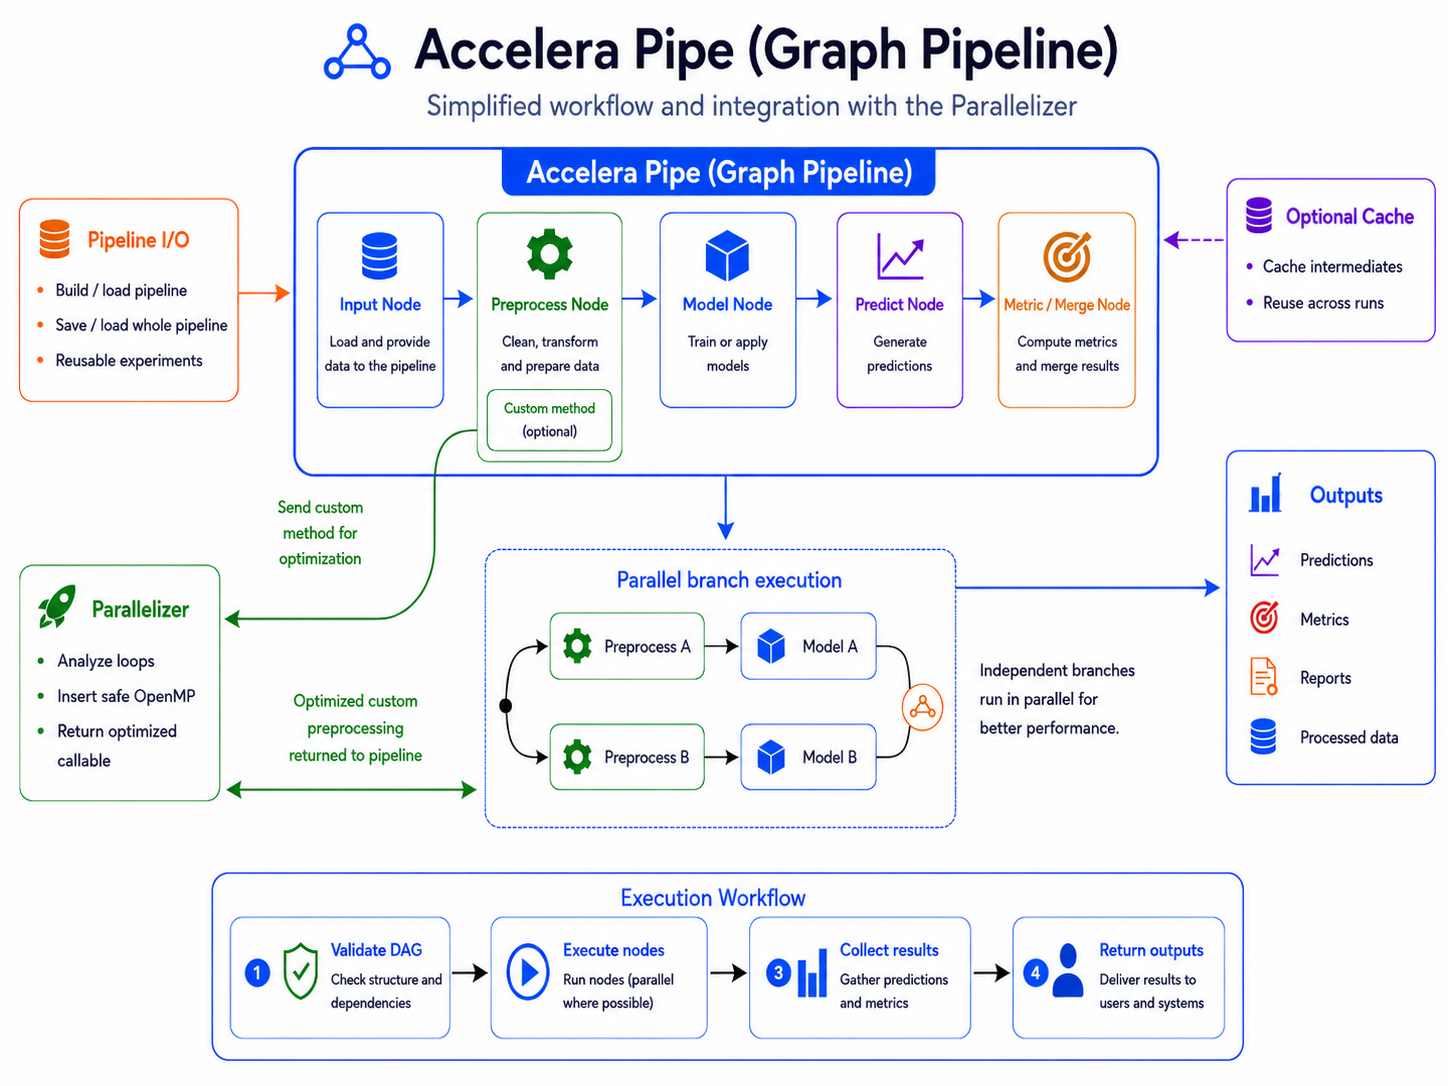
\includegraphics[width=\textwidth,keepaspectratio]{imgs/accelera_pipe.png}
\caption{Accelera Pipe workflow with custom preprocessing parallelization and pipeline reuse.}
\label{fig:accelera-pipe-workflow}
\end{figure}

The Accelera Pipe module is decomposed into two main layers: a Python API layer
and a native C++ graph execution layer. As shown in
Figure~\ref{fig:accelera-pipe-workflow}, the Python layer provides the user-facing
builder interface used to define preprocessing, model, prediction, metric, branch,
and merge nodes. It also handles metric wrapping, reports, serialization, save/load
support, and integration with the Code Parallelizer.

The native C++ layer manages the internal graph representation and execution
behavior. It stores nodes and edges, validates graph connections, computes the
topological execution order, schedules independent branches for parallel execution,
selects the final fitted path, and manages intermediate memory. When a preprocessing
node contains a supported custom method, Accelera Pipe can send it to the
Parallelizer, receive an optimized callable, and attach it back to the graph before
execution.

\begin{table}[H]
\centering
\small
\renewcommand{\arraystretch}{1.15}
\setlength{\tabcolsep}{4pt}
\caption{Main components of the Accelera Pipe module}
\label{tab:accelera-pipe-components}
\begin{tabular}{p{0.30\textwidth}p{0.62\textwidth}}
\toprule
\textbf{Component} & \textbf{Responsibility} \\
\midrule
Pipeline Builder Interface &
Provides the user-facing fluent API used to define preprocessing stages, models,
prediction steps, metrics, merge operations, and branches. It translates each user
call into a typed computational node instead of immediately executing the operation. \\
\midrule
Pipeline State and Persistence Manager &
Owns the native graph object, maps high-level node categories to graph node types,
controls graph execution settings, and provides save/load behavior for reusable
pipeline objects. \\
\midrule
Executed Graph Runtime &
Represents the fitted execution path selected after training. It allows the same
trained transformations and models to be reused for inference without keeping
unnecessary validation data or temporary training branches. \\
\midrule
Metric and Display Wrappers &
Adapt supervised metrics, unsupervised metrics, arrays, figures, dictionaries, and
reports into graph-compatible outputs that can be stored, selected, displayed, or
used in branch-selection strategies. \\
\midrule
Native Graph Engine &
Stores the pipeline as a directed acyclic graph, validates node connections, computes
execution order, schedules sequential or parallel execution, manages branch
selection, and controls intermediate-memory lifetime. \\
\midrule
Node Abstraction Layer &
Defines the common behavior of input, preprocessing, model, prediction, merge, and
metric nodes, including source-node relationships, stored data, GPU usage flags, and
selected-path markers. \\
\bottomrule
\end{tabular}
\end{table}

At the Python API level, each builder method creates or configures one graph
operation. A preprocessing node stores a function or transformer together with
execution parameters such as \texttt{execute\_fit} and \texttt{cache}. Before a
preprocessing function is stored, the module attempts to parallelize it through
\texttt{parallelizer.parallelize}. Model nodes store estimators, prediction nodes
store test data and the prediction method name, metric nodes store metric wrappers,
and merge nodes store the merge strategy.

\begin{table}[H]
\centering
\small
\renewcommand{\arraystretch}{1.15}
\setlength{\tabcolsep}{4pt}
\caption{Mapping from builder calls to graph node semantics}
\label{tab:accelera-pipe-builder-map}
\begin{tabularx}{\textwidth}{p{0.31\textwidth}p{0.18\textwidth}X}
\toprule
\textbf{Builder method} & \textbf{Node type} & \textbf{Main role} \\
\midrule
\texttt{preprocess(name, func)} &
\texttt{PREPROCESS} &
Transform input data or selected columns. \\
\midrule
\texttt{model(name, model)} &
\texttt{MODEL} &
Fit or apply a machine-learning estimator. \\
\midrule
\texttt{predict(name, test\_data)} &
\texttt{PREDICT} &
Run a model output function such as \texttt{predict}. \\
\midrule
\texttt{metric(name, metric)} &
\texttt{METRIC} &
Evaluate predictions using a supervised or unsupervised metric. \\
\midrule
\texttt{merge(name, strategy)} &
\texttt{MERGE} &
Combine outputs from multiple prediction branches. \\
\midrule
\texttt{branch(name, ...)} &
Multiple nodes &
Create alternative candidate paths in the DAG. \\
\bottomrule
\end{tabularx}
\end{table}

\subsection{Branching and Path Selection}

The native backend uses a graph abstraction rather than a linear pipeline. The
\texttt{Graph} class stores all nodes, tracks whether the graph has already been
compiled, supports cloning, and exposes methods for adding nodes, splitting
branches, executing, clearing, saving, loading, and enabling parallel execution.
The graph computes a topological execution order before running. This guarantees
that each node is executed only after its source nodes have produced their outputs.
If the graph contains branches, the execution result is followed by path selection
using one of the supported strategies: maximum metric, minimum metric, custom
strategy, or all paths.

\begin{lstlisting}[style=algostyle,caption={High-level Accelera Pipe training flow},label={alg:pipeline-training-flow}]
Input: training data X, optional labels y, graph G, selection strategy S
Output: predictions or metric results R, executed graph E

1:  Add X and y to the input node of G
2:  Compile G if its topological order is not already available
3:  Execute graph nodes sequentially or in parallel depending on G settings
4:  Collect outputs from final leaf nodes
5:  If G contains branches, select the path requested by S
6:  Clone the selected fitted path into a compact executed graph E
7:  Remove validation-only data and temporary training data
8:  Return R and E
\end{lstlisting}

Branching is handled by the native \texttt{split} operation. Each branch is converted
into a chain of graph nodes starting from the current leaf. If the current leaf node is
\(L\), then a branch \(B_i\) can be represented as:
\[
B_i = (L, n_{i1}, n_{i2}, \ldots, n_{ik})
\]
where \(n_{i1}, n_{i2}, \ldots, n_{ik}\) are the operations added to that branch.
A branch may contain a single node or a list of nodes, so the same mechanism supports
simple model comparison as well as full alternative sub-pipelines.

A useful optimization in branch construction is duplicate first-node sharing. If
several branches begin with the same first node, the graph creates that first node
once and connects the later branch consumers to its output. The sharing condition is:
\[
n_{11} = n_{21} = \cdots = n_{m1}
\]
where \(n_{i1}\) is the first node of branch \(B_i\). This is safe for the first
node because all such branches receive the same original input. The optimization is
deliberately conservative: later repeated nodes are not merged automatically because
their inputs may already differ due to earlier branch operations.

\begin{figure}[H]
\centering
\begin{minipage}{0.49\textwidth}
    \centering
    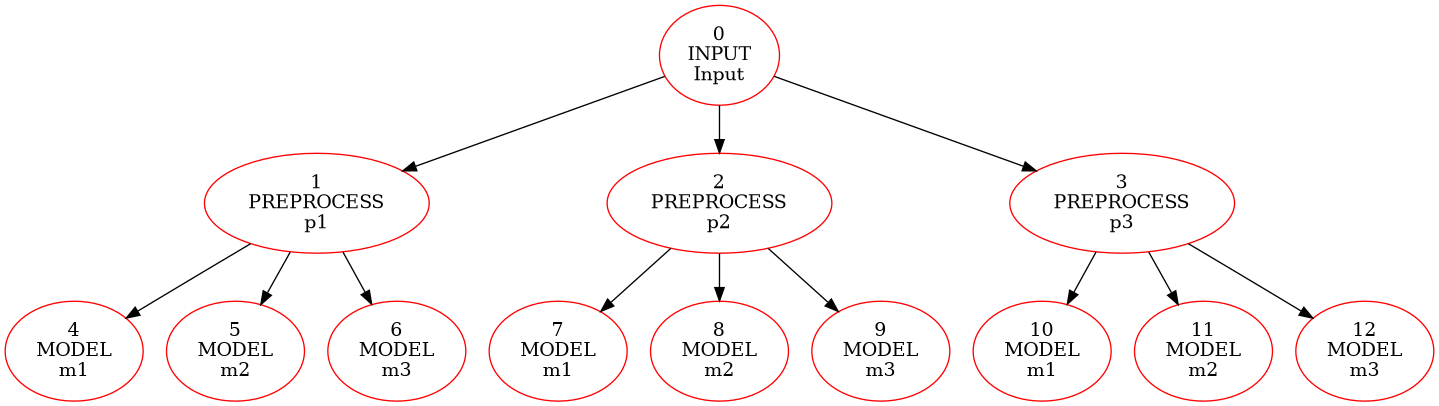
\includegraphics[width=\textwidth]{imgs/before_sharing.png}
    \caption{Before duplicate first-node sharing}
\end{minipage}
\hfill
\begin{minipage}{0.49\textwidth}
    \centering
    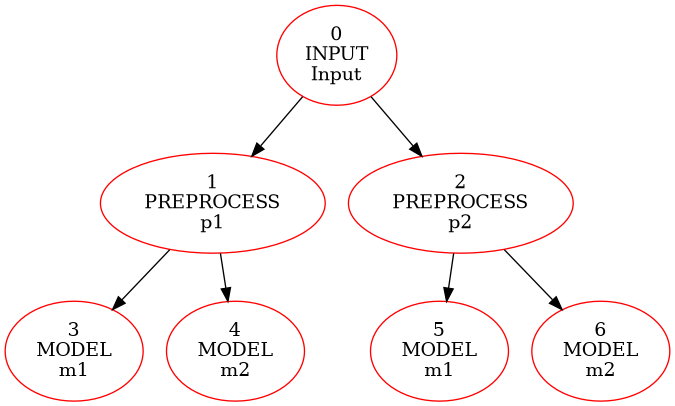
\includegraphics[width=\textwidth]{imgs/after_sharing.png}
    \caption{After duplicate first-node sharing}
\end{minipage}
\end{figure}

\subsection{Intermediate Memory Management}

Machine-learning pipelines can produce large intermediate arrays, especially when
several preprocessing branches are evaluated. Accelera Pipe therefore tracks
remaining consumers for each node output. Once the last downstream consumer finishes,
the corresponding intermediate data can be released. Model and metric nodes are
treated more carefully because they may hold fitted estimators or evaluation state,
while input and preprocessing data can often be cleared after their consumers are
done. This policy reduces memory pressure without changing the logical result of the
graph.

\begin{lstlisting}[style=algostyle,caption={Consumer-count based intermediate release},label={alg:consumer-release}]
Input: executed node N, remaining consumer table C
Output: graph with unused temporary data released

1:  for each source node S that feeds N do
2:      C[S] = C[S] - 1
3:      if C[S] == 0 and S is releasable then
4:          clear the temporary data stored by S
5:      end if
6:  end for
\end{lstlisting}

The consumer-count mechanism is used after each node finishes executing. Every
source node keeps a counter representing how many downstream nodes still need
its output. For a source node \(S\), the remaining-consumer count can be written as:
\[
C(S) = |\{N \mid S \rightarrow N \text{ and } N \text{ has not executed yet}\}|
\]
When a downstream consumer completes, the counter is decreased:
\[
C(S) \leftarrow C(S) - 1
\]
If the counter reaches zero and the source node is safe to clear, the temporary output
is released. This allows the graph to reduce memory pressure during branch-heavy
training runs without changing the final predictions or selected path.

\subsection{Parallel Graph Execution}
The graph can run independent nodes in parallel, but a node can start only after all
its parents have finished. For any node \(N\), the readiness condition is:
\[
\text{ready}(N) \Longleftrightarrow \forall P \in \text{Parents}(N),\; \text{finished}(P)=\text{true}
\]
The backend uses CPU thread semaphores, a separate GPU semaphore, and dependency
checks over the topological order. This prevents a downstream node from reading
incomplete data and also serializes GPU work when necessary. CPU nodes are allowed
to execute concurrently as long as worker slots are available, while GPU nodes are
handled more conservatively using a single execution slot. This makes the scheduler
safe for mixed CPU/GPU graphs without changing the dependency semantics. This also
allows the graph to use available hardware more efficiently when several branches are
ready at the same time. At the same time, synchronization keeps the final execution
result equivalent to a valid sequential topological run. The number of CPU threads is
based on hardware concurrency but can be overridden using the
\texttt{ACCELERA\_NUM\_THREADS} environment variable.

\newpage
\begin{lstlisting}[style=algostyle,caption={Parallel graph execution scheduling},label={alg:parallel-graph-execution}]
Input: topological execution order T
Output: completed graph execution or reported error

1:  Initialize finished and started state for all nodes
2:  Build remaining-consumer counts for intermediate outputs
3:  Create limited CPU worker slots and one GPU execution slot
4:  while unfinished nodes still exist do
5:      for each node N in T do
6:          if N has not started and all parent nodes are finished then
7:              Acquire a CPU slot or the GPU slot depending on N
8:              Mark N as started
9:              Launch N asynchronously
10:             After N finishes:
11:                 Mark N as finished
12:                 Release unused source outputs
13:                 Release the CPU or GPU slot
14:          end if
15:      end for
16:  end while
17:  Wait for all launched tasks
18:  Rethrow any stored node execution error
\end{lstlisting}

Algorithm~\ref{alg:parallel-graph-execution} describes the runtime scheduling idea
implemented by the native graph backend. The graph is already arranged in
topological order, but the scheduler does not simply execute nodes one by one.
Instead, it repeatedly searches for nodes whose parents have finished and launches
them asynchronously when a CPU or GPU execution slot is available. CPU nodes share
a limited pool of worker slots, while GPU nodes use a separate single-slot semaphore
to avoid unsafe concurrent GPU execution. After a node completes, the backend marks
it as finished, releases any temporary source outputs that are no longer needed, and
signals the scheduler so that newly ready child nodes can start. Any exception raised
inside a node is stored and rethrown after all launched tasks are joined, which gives a
clear error message containing the failed node name and whether it was executed as a
CPU or GPU node.


\subsection{Design Constraints}

The Accelera Pipe module has several design constraints that guide how the graph
is constructed, executed, and reused. The first constraint is that the internal
workflow must always remain a valid directed acyclic graph. Since execution
depends on topological ordering, cyclic dependencies are not allowed. For any
edge from node \(u\) to node \(v\), the execution order must satisfy:
\[
u \rightarrow v \Rightarrow \tau(u) < \tau(v)
\]
where \(\tau\) represents the topological order of the graph. This guarantees
that every node is executed only after its required source nodes have already
produced their outputs.

The second constraint is node-type validity. Not every node can be connected to
any other node. For example, a prediction node must follow a model node, a metric
node must follow a prediction or merge node, and a merge node should combine
compatible prediction outputs. These restrictions preserve the semantic meaning
of the pipeline and prevent invalid workflows from reaching the execution stage.

The third constraint is safe memory management. Since branch-heavy workflows can
produce many temporary arrays, the backend must release intermediate data only
when it is no longer needed. For a source node \(S\), the remaining-consumer
count is:
\[
C(S) = |\{N \mid S \rightarrow N \text{ and } N \text{ has not executed yet}\}|
\]
The output of \(S\) can be cleared only when \(C(S)=0\) and the node is safe to
release. This reduces memory pressure without changing the final selected path
or prediction results.

The fourth constraint is parallel execution safety. Independent nodes may run in
parallel, but a node can start only after all of its parent nodes have completed:
\[
\text{ready}(N) \Longleftrightarrow \forall P \in \text{Parents}(N),\;
\text{finished}(P)=\text{true}
\]
This prevents downstream nodes from reading incomplete data. The backend also
uses limited CPU worker slots and a separate GPU slot to avoid unsafe resource
sharing during execution.

Finally, the executed graph must not retain training-only data. After training,
the selected path is cloned into an \texttt{ExecutedGraph}, validation inputs are
removed, metric targets are cleared, and temporary arrays are released. This
keeps the saved inference graph compact and focused only on fitted
transformations and models.


\subsection{Summary}
The Accelera Pipe module also supports persistence. The Python \texttt{PipelineBase}
class saves and loads pipeline objects using pickle, while the C++ graph exposes
its state as a Python dictionary containing node information, selected-path flags,
source indices, cached data, graph compilation state, and parallel execution
configuration. During loading, the graph rebuilds the nodes and reconnects them
using the stored source indices, making the native graph serializable.

The module can also export a graph-like representation of the pipeline structure.
The graph utility code writes an XML-style network description containing layers
for input, preprocessing, model, prediction, merge, and metric nodes, together
with their edges. This representation is useful for debugging, visualization,
and understanding the executable graph generated from the high-level pipeline.

In summary, Accelera Pipe is a hybrid Python/C++ pipeline execution system.
Python provides the user-facing construction interface, while C++ provides graph
semantics, execution scheduling, branch selection, memory-lifetime control, and
parallel execution support, keeping the module both efficient and easy to use.


\section{Code Parallelizer Module}

\subsection{Functional Description}

The Code Parallelizer module is responsible for transforming supported loop-heavy
source code into optimized C++ code annotated with OpenMP pragmas. It is designed
to reduce the execution time of custom preprocessing functions and standalone code
snippets by identifying loops that can be safely executed in parallel. The module
accepts different input forms: a file path, a source string, a custom Python function,
or a custom transformer instance. Regardless of the input form, the scientific goal is
the same: normalize the input into a C++ loop-analysis path, detect parallelization
opportunities, and return either parallelized source code or a compiled
Python-callable native function.

This process can be viewed as a transformation from an original program \(P\) into
an optimized program \(P'\):
\[
P' = \mathcal{T}(P)
\]
where \(\mathcal{T}\) represents the parallelization pipeline, including source
normalization, loop extraction, loop classification, safety validation, and OpenMP
pragma insertion. If no safe optimization is found, the transformation keeps the
program behavior unchanged by returning the original code or callable.

For Python input, the module first lowers a restricted Python subset into C++. This
conversion is intentionally limited to predictable language constructs such as
arithmetic expressions, assignments, \texttt{for range(...)} loops, conditionals,
function definitions, array-style indexing, and simple calls. The resulting C++ code is
then analyzed by the same loop extraction path used for native C/C++ input. This
design avoids building two separate parallelization pipelines and ensures that both
Python and C++ inputs are judged using the same loop features and safety checks.

After normalization, the module extracts candidate loops and checks whether each loop
can be parallelized safely. For a loop \(L_i\), the final decision can be represented as:
\[
d_i \in \{\text{sequential},\; \text{parallel\_for},\; \text{reduction}\}
\]
where \(\text{sequential}\) means that the loop is left unchanged,
\(\text{parallel\_for}\) means that a normal OpenMP parallel loop pragma can be
inserted, and \(\text{reduction}\) means that the loop can be parallelized using an
OpenMP reduction clause. This decision is based on both learned classification and
rule-based safety checks, so the module does not rely only on a model prediction when
program correctness may be affected.

\begin{table}[H]
\centering
\small
\renewcommand{\arraystretch}{1.15}
\setlength{\tabcolsep}{4pt}
\caption{Supported operations in the Python-to-C++ converter}
\begin{tabular}{p{0.27\textwidth}p{0.60\textwidth}}
\toprule
Category & Supported forms and notes \\
\midrule
Constants and names & \texttt{None}, booleans, integers, floats, strings, and variables. \\
\midrule
Arithmetic & Addition, subtraction, multiplication, division, modulo, and power using \texttt{std::pow}. \\
\midrule
Unary and boolean & Unary plus, unary minus, logical not, logical and, and logical or. \\
\midrule
Comparisons & Equality, inequality, less-than, less-than-or-equal, greater-than, and greater-than-or-equal; chained comparisons rejected. \\
\midrule
Calls and printing & Ordinary function calls and \texttt{print}; keyword arguments are generally unsupported. \\
\midrule
Access operations & Attribute access and indexing are supported; slicing is rejected. \\
\midrule
Assignment & Single-target assignment and indexed assignment are supported; multi-target assignment is rejected. \\
\midrule
Augmented assignment & Simple-name \texttt{+=}, \texttt{-=}, \texttt{*=}, \texttt{/=}, and \texttt{\%=}. \\
\midrule
Control flow & \texttt{if}/\texttt{else} blocks and \texttt{return} statements. \\
\midrule
Loops & \texttt{for i in range(...)} loops with one, two, or three range arguments. \\
\midrule
Functions & Function definitions are emitted as C++ template-style functions; decorators are rejected. \\
\bottomrule
\end{tabular}
\end{table}

After normalization, the module extracts loop information using native Clang AST
bindings. Each loop is represented by its source code and source-line range. The
Python orchestration layer then computes a fixed loop-feature representation,
uses a classifier endpoint to predict whether the loop is a parallelization
candidate, and validates the decision with rule-based checks. If the loop is
safe, the module injects an OpenMP directive such as
\texttt{\#pragma omp parallel for}. For reduction-like loops, it can also emit a
reduction clause when the reduction variable is valid.

The module has a fail-safe behavior. If the input cannot be converted, analyzed,
classified, compiled, or loaded as a native extension, the system falls back to
the original Python function or leaves the code unmodified. This is important
because parallelization is an optimization, not a reason to change the semantic
meaning of the user's program.

\subsection{Modular Decomposition}

The Code Parallelizer module is decomposed into six cooperating components:
input normalization, Python-to-C++ conversion, Clang-based loop extraction,
feature extraction and vectorization, classification with rule-based validation,
and OpenMP/native-extension generation.

\begin{table}[H]
\centering
\small
\renewcommand{\arraystretch}{1.15}
\setlength{\tabcolsep}{4pt}
\fontsize{8.8}{10.5}\selectfont
\caption{Main components of the Code Parallelizer module}
\begin{tabular}{p{0.27\textwidth}p{0.63\textwidth}}
\toprule
Component & Responsibility \\
\midrule
Parallelization Orchestrator & Receives source strings, file paths, custom functions, and transformer instances. It coordinates conversion, loop extraction, feature analysis, classification, pragma insertion, caching, compilation, and fallback behavior. \\
\midrule
Input Normalization Layer & Converts accepted input forms into a common source-analysis representation. Files are read, source strings are analyzed directly, functions are captured from source, and transformer instances are inspected through their transformation method. \\
\midrule
Python-to-C++ Converter & Translates a restricted subset of Python into C++ so Python preprocessing logic can enter the same static loop-analysis pipeline as native C/C++ code. \\
\midrule
Loop Extraction Engine & Uses a compiler-style front end to locate loops, record source ranges, and expose structured loop information for feature extraction and rewriting. \\
\midrule
Feature Extraction and Embedding Generator & Computes structural, dependency, memory-access, control-flow, arithmetic, and reduction features, then maps them into a fixed-size numeric representation. \\
\midrule
Parallelization Classifier and Safety Resolver & Combines classifier predictions with deterministic safety rules to decide whether a loop remains sequential, receives a parallel-for pragma, or receives a reduction pragma. \\
\midrule
OpenMP Rewriter & Inserts the selected OpenMP directive while avoiding unsafe duplicate insertion, especially when an outer loop already contains selected inner loops. \\
\midrule
Native Compilation and Loading Layer & Wraps optimized C++ into a Python-callable extension, adds OpenMP flags only when needed, builds the native module, loads it at runtime, and returns the optimized callable. \\
\midrule
Caching Layer & Stores processed source and compiled native functions using source-based hashes to avoid repeated conversion and compilation. \\
\bottomrule
\end{tabular}
\end{table}

Figure~\ref{fig:parallelizer_workflow} summarizes the overall data flow. In general, 
supported inputs are normalized into a common C++ loop-analysis path, 
while callable Python inputs additionally proceed to PyBind11 extension generation.

\begin{figure}[H]
\centering
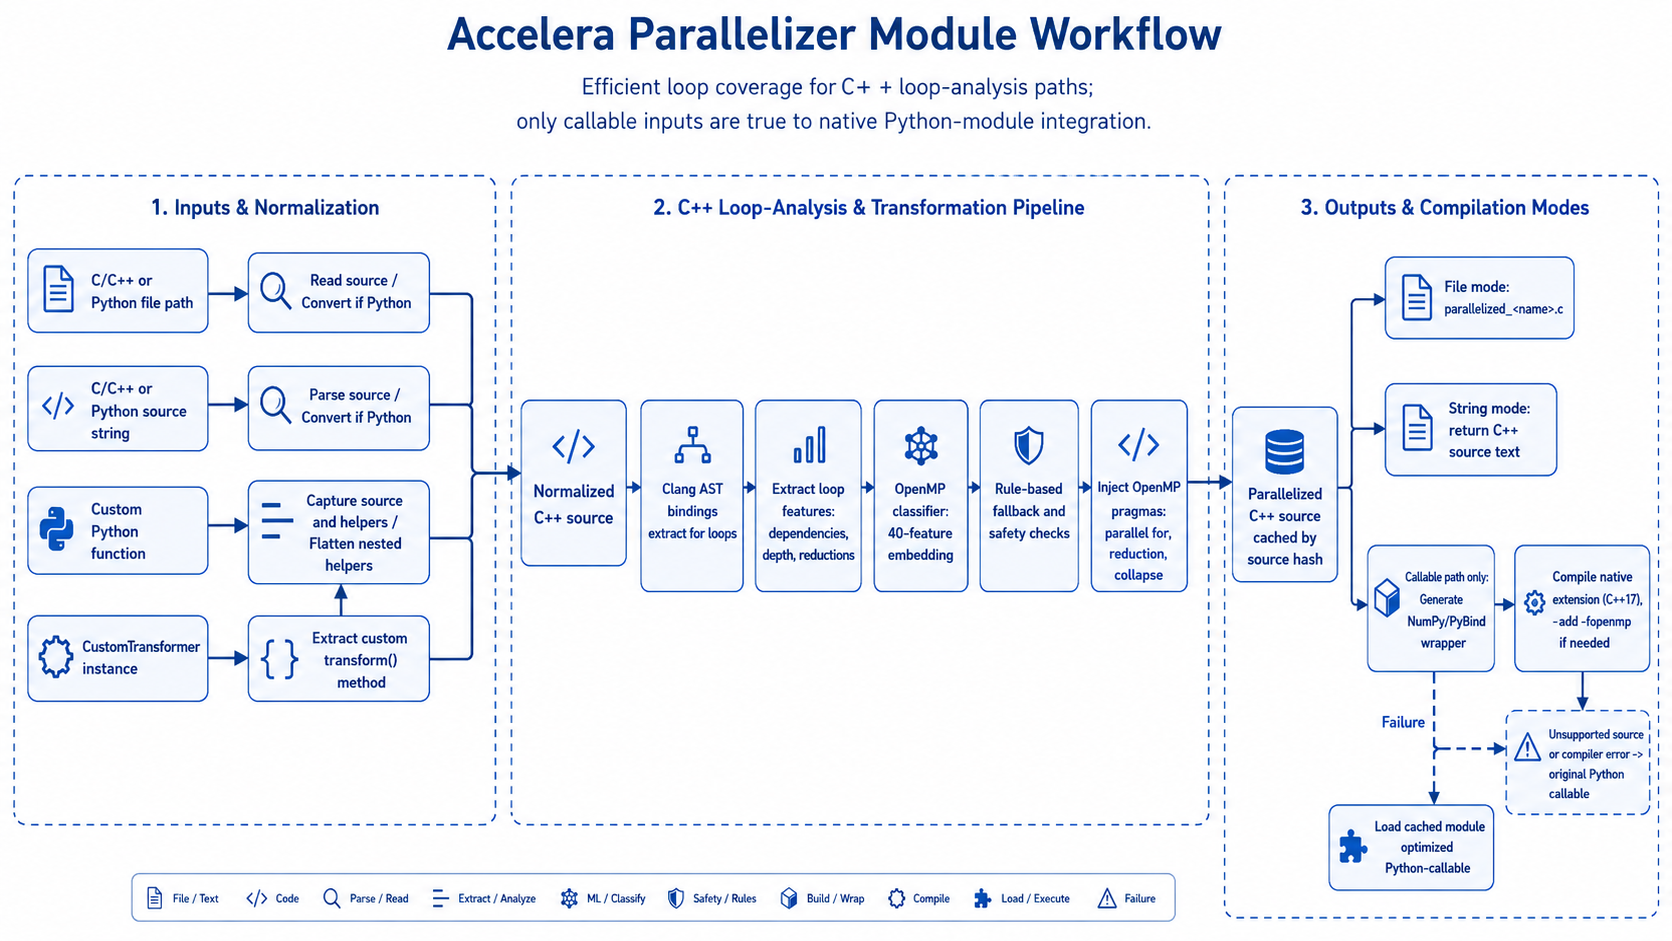
\includegraphics[width=\textwidth,keepaspectratio]{imgs/pp.png}
\caption{Code Parallelizer module workflow}
\label{fig:parallelizer_workflow}
\end{figure}

The feature extraction stage analyzes both code structure and loop behavior, 
including reductions, array accesses, dependencies, indirect memory access, early exits, 
nesting depth, branches, function calls, arithmetic operations, and vectorization potential. 

These indicators are encoded into a 40-dimensional vector for the classifier, 
then refined by deterministic safety rules that can still detect safe cases such as reductions, 
independent array writes, and nested loop patterns.

\begin{lstlisting}[style=algostyle,caption={Loop classification and pragma insertion}]
Input: source program P
Output: source program P' with safe OpenMP pragmas

1:  if P is Python source then
2:      convert the supported Python subset into C++
3:  end if
4:  Extract for-loops using the Clang AST frontend
5:  for each extracted loop L do
6:      compute structural, memory, dependency, and reduction features
7:      send the 40-feature vector to the classifier service
8:      combine the predicted class with rule-based safety checks
9:      if the resolved class is parallel_for then
10:         insert #pragma omp parallel for
11:     else if the resolved class is reduction then
12:         insert #pragma omp parallel for reduction(...)
13:     else
14:         leave the loop unchanged
15:     end if
16: end for
17: Cache and return the transformed source code
\end{lstlisting}

The compilation path is used when the input is a Python callable. The
parallelizer extracts or receives the function source, converts it to C++,
parallelizes the C++ loop body, wraps the result in a PyBind11 module, compiles
it as a shared native extension, loads the extension, and returns the optimized
function. Caching is used at both the transformed-source level and the compiled
method level. The cache key includes the compilation cache version, the function
name, the compiler optimization level, the extension suffix, and the source
code. This prevents recompiling the same function repeatedly.

\subsection{Design Constraints}

The most important design constraint of the Code Parallelizer is correctness.
OpenMP pragmas can improve performance, but an incorrect pragma can produce
wrong numerical results. Therefore, classifier output is not applied blindly.
The module applies additional safety rules to avoid unsafe transformations when
there are loop-carried dependencies, indirect accesses, early exits, side-effect
function calls, or invalid reduction variables. Inner loops are also skipped when
an outer selected loop already covers their range, preventing nested duplicate
pragma insertion.

The second constraint is the restricted Python subset. Full Python semantics are
too dynamic to translate safely into C++ using a lightweight source converter.
The converter therefore rejects unsupported syntax such as decorators, slicing,
chained comparisons, unsupported operators, non-range loop iterators,
multi-target assignment, complex dynamic dispatch, and unsupported expression
forms. This restriction is not a weakness in the design; it is a correctness
boundary. The system optimizes code only when it can produce predictable C++.

The third constraint is compiler and platform compatibility. Native callable
optimization depends on a working C++ compiler, Python include paths, PyBind11
headers, NumPy-compatible array wrapping, and platform-specific shared extension
suffixes. The compiler path uses C++17 and adds \texttt{-fopenmp} only when the
parallelized code actually contains OpenMP pragmas. On non-Windows platforms it
also uses position-independent code flags suitable for shared libraries. If
compilation fails, the original Python callable is returned.

The fourth constraint is input and output compatibility. The current compiled
callable path is oriented toward functions with one named input parameter and
NumPy-like two-dimensional numeric data. The wrapper rewrites array access to
PyBind11 unchecked NumPy access and exposes the compiled function back to
Python. This makes the generated extension useful for numeric preprocessing
loops, but it also means that arbitrary Python functions with complex object
structures are outside the supported optimization target.

The fifth constraint is reproducibility and caching. Because native compilation
can be expensive, the module caches processed C++ code and compiled functions
using source hashes. The cache must include enough information to avoid stale or
incorrect reuse when compiler options, cache version, function name, source code,
or extension suffix changes. This design improves repeated execution time while
keeping cache invalidation explicit.

\subsection{Summary}

The Code Parallelizer is directly integrated with Accelera Pipe. When a
preprocessing node is added, the pipeline calls the parallelizer before storing
the preprocessing object. If the object is a custom Python function, it is wrapped
as a source-backed function whose runtime callable can be replaced by the
compiled implementation. If the object is a custom transformer instance, the
parallelizer attempts to optimize its \texttt{transform} method and attach the
optimized method back to the instance. If the object is a library transformer or
an unsupported callable, it is returned unchanged.

\begin{figure}[H]
\centering
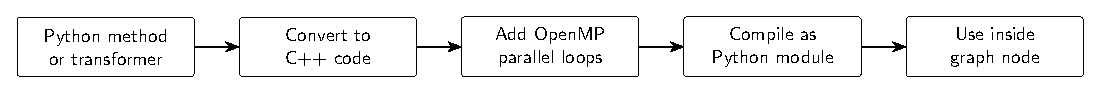
\includegraphics[width=\textwidth]{imgs/parallelizer_accelera_pipe_flow.pdf}
\caption{Integration flow for compiled preprocessing inside Accelera Pipe}
\end{figure}

Scientifically, the final design uses a hybrid approach rather than a purely
generative code model. An earlier generator-based design attempted to emit
parallelized code using a neural sequence model. That approach was rejected
because the dataset size was not sufficient for reliable sequence generation and
because generated synthetic samples risked introducing distribution bias. The
current design is more controlled: the classifier only predicts the type of
parallelization opportunity, while deterministic compiler-like rules decide how
and whether the pragma is inserted. This separation makes the system easier to
inspect, easier to debug, and safer for user code.

Overall, the Code Parallelizer acts as an optimization layer around user-defined
numeric loops. It does not attempt to parallelize all Python programs. Instead,
it targets the subset where static analysis, feature extraction, classifier
prediction, rule validation, and native compilation can cooperate safely. This
fits the broader Accelera design philosophy: keep the Python API simple, but move
performance-sensitive and structurally analyzable work into optimized native
execution when the system can do so without changing program semantics.

\section{Auto Preprocessing Module}
\noindent The Auto Preprocessing module is responsible for automating the data
understanding, exploratory data analysis, and preprocessing stages of the data
science workflow. The module was designed to reduce repeated manual work and to
prepare different types of datasets before model training.
\begin{figure}[H]
    \centering
    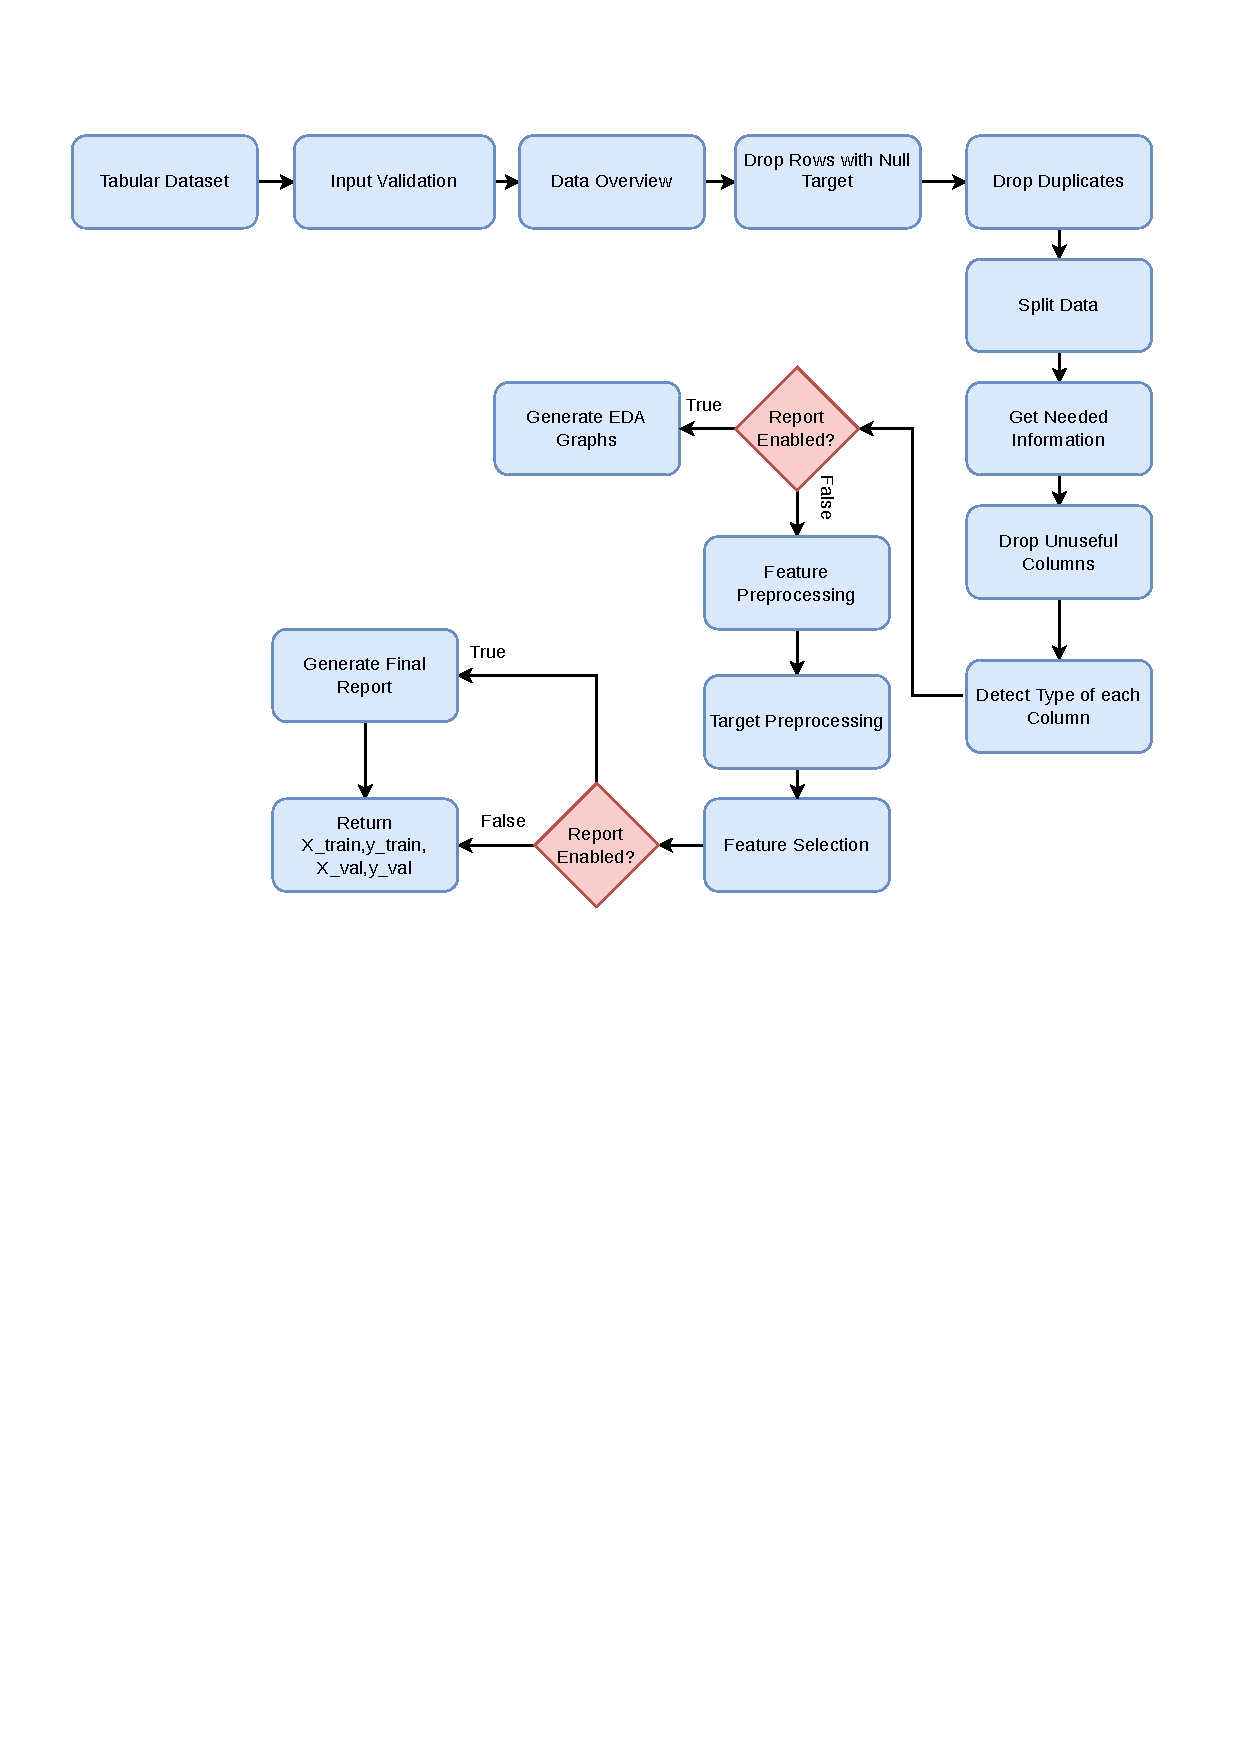
\includegraphics[width=1\textwidth]{imgs/tabular.pdf}
    \caption{Tabular Preprocessing Workflow}
    \label{fig:tabular_preprocessing_workflow}
\end{figure}
\begin{figure}[H]
    \centering
    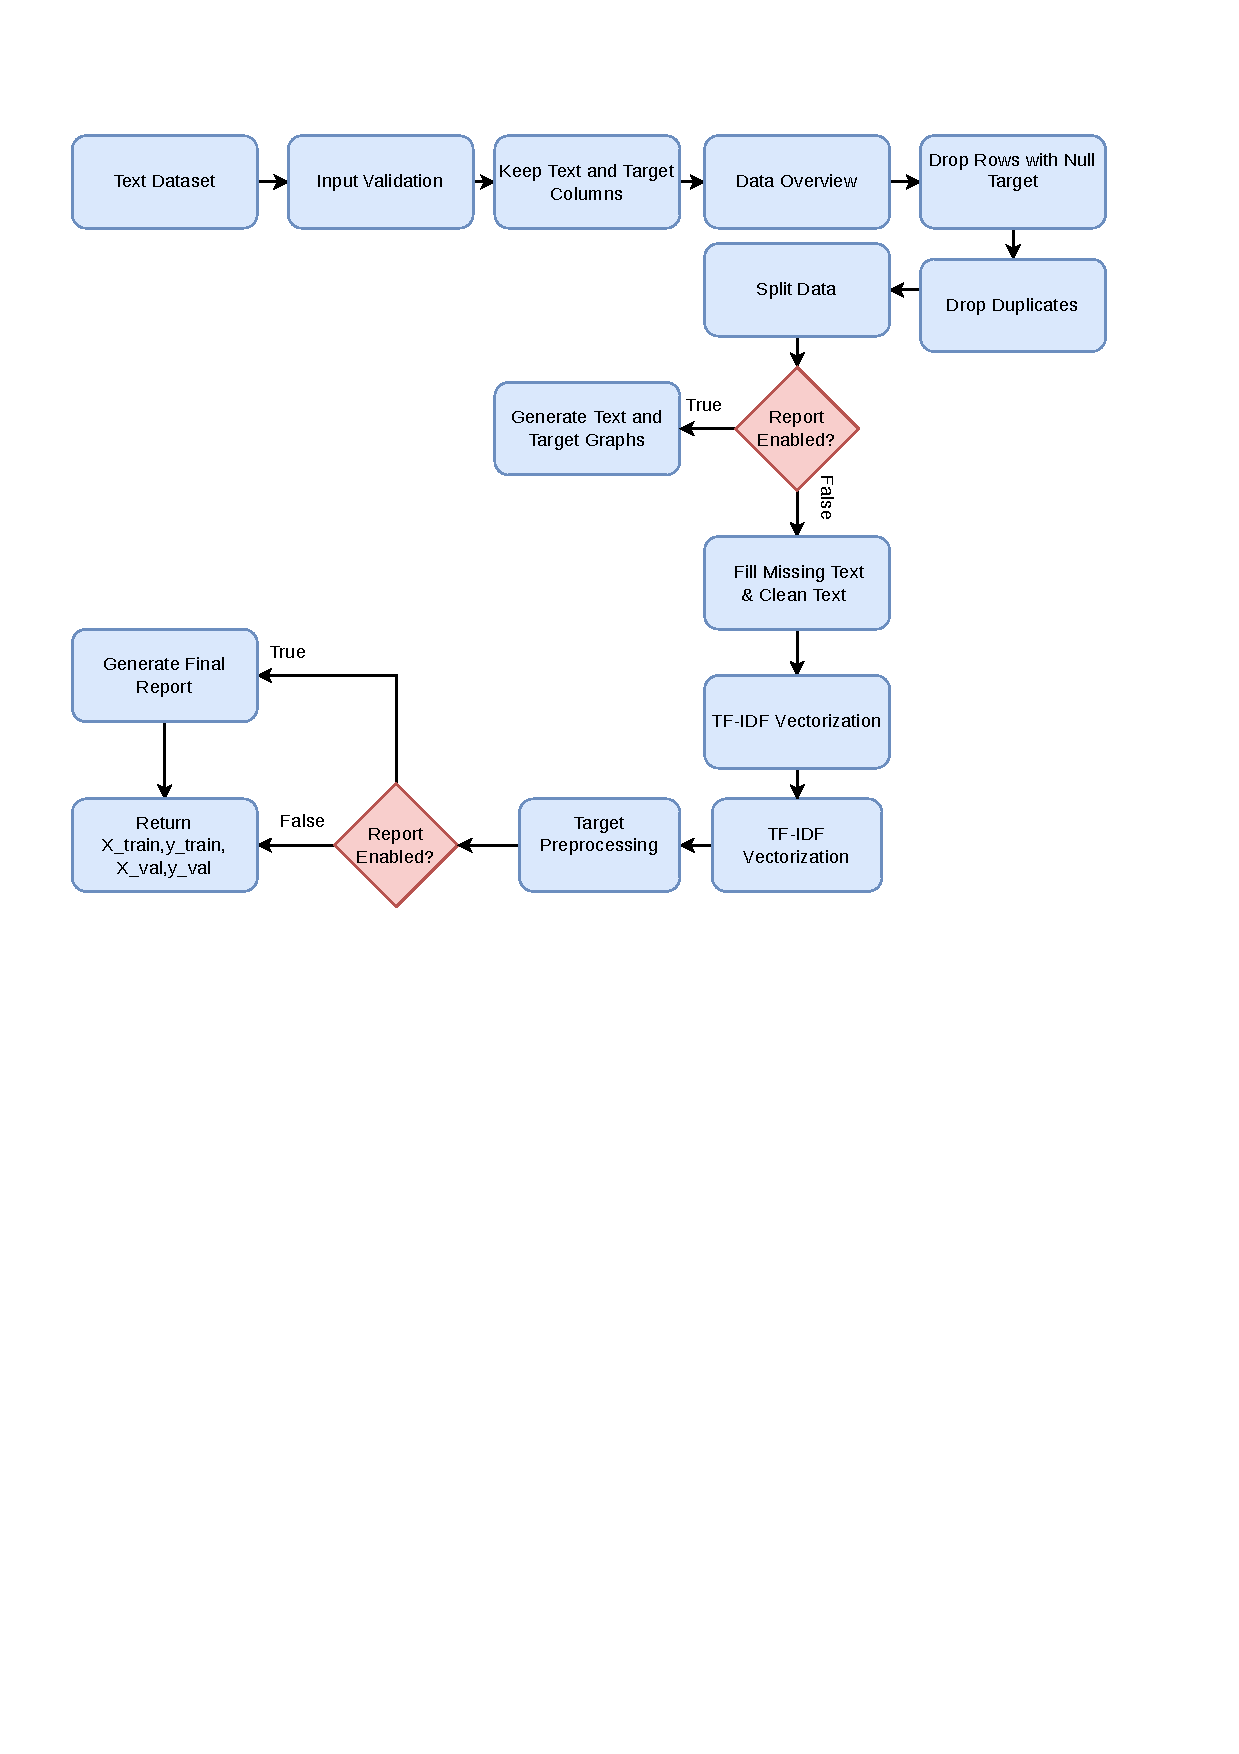
\includegraphics[width=1\textwidth]{imgs/text.pdf}
    \caption{Text Preprocessing Workflow}
    \label{fig:text_preprocessing_workflow}
\end{figure}
\begin{figure}[H]
    \centering
    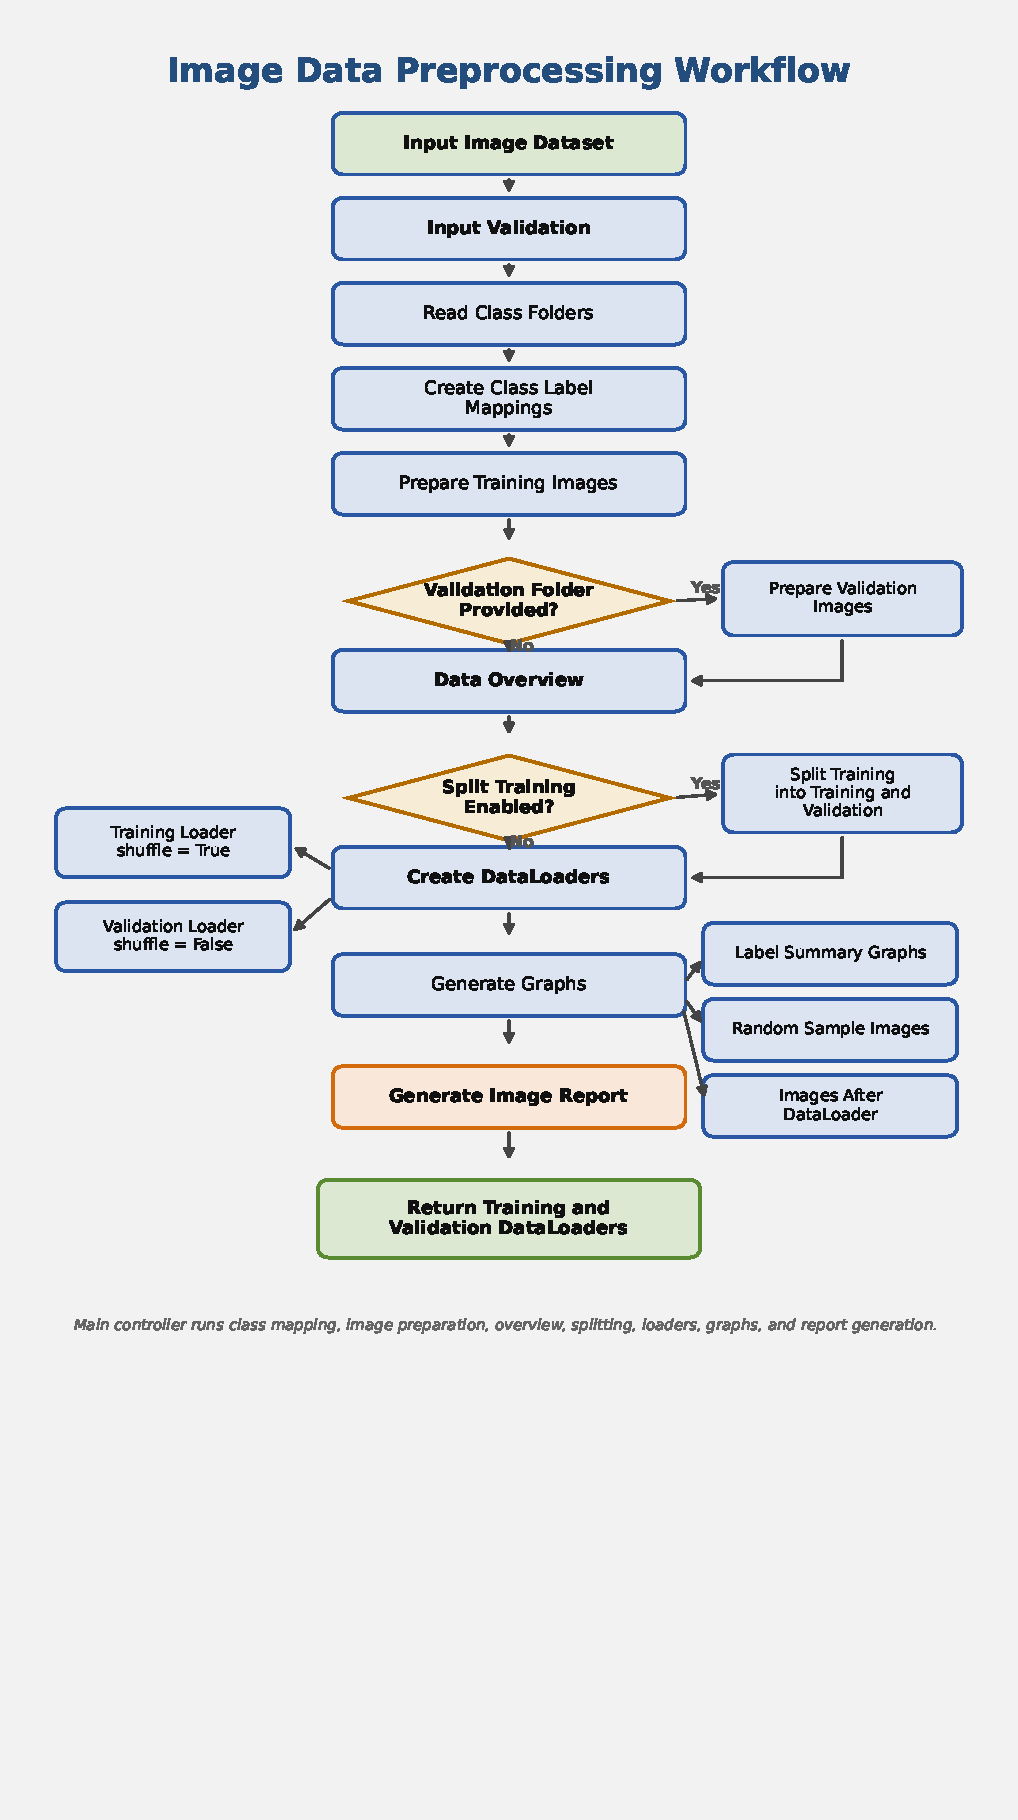
\includegraphics[width=1\textwidth]{imgs/image_workflow.pdf}
    \caption{Image Preprocessing Workflow}
    \label{fig:image_preprocessing_workflow}
\end{figure}
\subsection{Functional Description}
\noindent The main function of this module is to receive a dataset and user configuration,
then return processed data that is ready for machine learning or deep learning
models. The module supports tabular, text, and image datasets.
\noindent The module also generates a report when this option is enabled. The report
summarizes information about the dataset and the preprocessing steps applied.

\subsubsection{Tabular datasets}
\noindent For tabular datasets it supports both classification and regression
tasks. It analyzes the dataset, removes duplicate records, splits the data into
training and validation sets, detects column types, handles missing values,
encodes categorical features, scales numerical features, applies target
preprocessing, performs feature selection, and saves the preprocessing objects
needed later for test data.
\subsubsection{Text datasets}
\noindent It supports classification tasks. It cleans the text,
tokenizes it, applies text preprocessing steps, and converts the text into a
numerical representation suitable for machine learning models.
\subsubsection{Image datasets}
\noindent It supports image classification by reading images from class
folders, validating image files, resizing images, applying augmentation, normalizing pixel values, and
preparing the data loaders needed for training.




\subsection{Modular Decomposition}
\noindent The Auto Preprocessing module is divided based on the type of input data. The
system supports three main types of data: tabular data, text data, and image data.
Each type has its own preprocessing workflow and functions because every data type has a different
structure and needs different techniques.

\subsubsection{Tabular Data Preprocessing Functions}


\begin{description}
    \item[\texttt{\_\_init\_\_():}]
    This is the constructor that receives the dataset and the user settings. 
    It validates these settings before starting the preprocessing process. 
    \item[\texttt{handel\_bool\_types():}]
    This function handles columns that have bool data type. It finds the columns that have
    boolean values and converts them into integer values.

    \item[\texttt{data\_overview():}]
    This function gives a general overview of the dataset before preprocessing.
    \item[\texttt{drop\_target\_nulls():}]
    This function drops rows have null value in the target.

    \item[\texttt{drop\_duplicates():}]
    This function removes repeated rows from the dataset.

    \item[\texttt{split\_data():}]
    This function splits the dataset into training and validation sets. The split is
    based on the validation size and random state selected by the user. The output of
    this function is \texttt{X\_train}, \texttt{X\_val}, \texttt{y\_train}, and
    \texttt{y\_val}.

    \item[\texttt{get\_data\_info():}]
    This function studies each column in the training data. It collects important
    information such as data type, number of unique values,
    missing values, and missing percentage. For numerical columns, it also calculates the mean,and median.

    \item[\texttt{is\_drop\_column():}]
    This function decides whether a column should be removed or kept. A column is
    removed if it is included in the user selected drop list, if it has only one constant
    value, or if its missing value percentage is higher than the selected threshold. 
    \item[\texttt{drop\_col():}]
    This function removes the selected columns from both the training and validation
    datasets. It also saves the dropped columns and their reasons in a file. This helps
    the system apply the same dropping step later on testing or new data.

    \item[\texttt{detect\_column\_types():}]
    This function detects the type of each feature. This step is important because each
    feature type needs a different preprocessing method. The features are divided into
    binary columns, ordinal columns, numerical columns, continuous columns,
    low cardinality categorical columns, high cardinality categorical columns, and
    unsupported columns. The function also stores the preprocessing steps for each
    column to be shown later in the report.
    \begin{table}[H]
    \centering
    \caption{Detected Column Types in Tabular Data}
    \label{tab:feature_types}
    \begin{tabular}{|p{3.5cm}|p{7cm}|p{4cm}|}
    \hline
    \textbf{Feature Type} & \textbf{Description} & \textbf{Examples} \\
    \hline

    Binary &
    Columns containing exactly two unique values. &
    yes/no, 1/0 \\
    \hline

    Ordinal &
    Integer columns with a small number of unique values less than or equal to
    \texttt{max\_ordinal\_unique}. &
    Ratings or levels such as 1, 2, 3, 4 \\
    \hline

    Numerical &
    Integer columns with a number of unique values greater than
    \texttt{max\_ordinal\_unique}. &
    Age, number of transactions \\
    \hline

    Continuous &
    Floating-point columns. &
    Height = 175.5, price = 19.99, temperature = 36.6 \\
    \hline

    Low Cardinality Categorical &
    Object or string columns with a number of unique values less than or equal to
    \texttt{cardinality\_threshold}. &
    Product categories, gender, country group \\
    \hline

    High Cardinality Categorical &
    Object or string columns with a number of unique values greater than
    \texttt{cardinality\_threshold}. &
    Product names, cities \\
    \hline

    Other &
    Columns with unsupported or non-standard data types. These columns are excluded from
    the preprocessing pipeline. &
    Dates, complex objects, unsupported formats \\
    \hline

    \end{tabular}
    \end{table}



    \item[\texttt{make\_graphs():}]
    This function creates graphs when the report option is enabled. The type of graph
    depends on the feature type and the problem type.

    \item[\texttt{features\_preprocessing():}]
    This function applies the preprocessing steps to the input features. It creates
    different pipelines based on the detected feature types:
    \begin{itemize}
        \item Numerical and continuous features are filled using the median and scaled
        using robust scaling.
        \item Binary features are filled using the most frequent value and encoded using
        ordinal encoding.
        \item Low cardinality categorical features are filled using the most frequent
        value and encoded using binary encoding.
        \item High cardinality categorical features are filled using the most frequent
        value and encoded using frequency encoding.
        \item Ordinal features are filled using the most frequent value and scaled using
        robust scaling.
    \end{itemize}
    These pipelines are combined using \texttt{ColumnTransformer}. The transformer is
    fitted on the training data and then applied to the validation data. The fitted
    preprocessor and the generated feature names are saved for later use.

    \item[\texttt{target\_preprocessing():}]
    This function prepares the target column based on the problem type. For
    classification label encoding is used to convert class labels into numbers. For regression robust scaling is applied. The target
    preprocessor is saved so the same transformation can be used later.

    \item[\texttt{features\_importance():}]
    This function selects the most useful features using mutual information. Only features with scores
    greater than or equal to the selected threshold are kept. The selected features are
    saved in a file to use it in the inference step. 
    \item[\texttt{common\_preprocessing():}]
    This is the main function that controls the full tabular preprocessing workflow. It
    calls the previous functions in order. It starts by handling boolean columns,
    generating the data overview,drop rows have null target, removing duplicates, and splitting the data. Then, it
    extracts column information, drops unsuitable columns, detects column types,
    generates graphs, preprocesses the features, preprocesses the target, applies feature
    selection, and generates the report if enabled.It returns the processed
    training and validation data.
\end{description}

\subsubsection{Text Data Preprocessing Functions}


\begin{description}
    \item[\texttt{\_\_init\_\_():}]
     This is the constructor that receives the dataset and the user settings. 
     It validates these settings before starting the preprocessing process.Also removes any columns that are not the text column or the target
     column. This keeps only the columns needed for text classification. It also
    downloads the required NLTK resources, such as \texttt{punkt} and
    \texttt{stopwords}.
    \item[\texttt{make\_graphs():}]
    This function creates graphs if the report option is enabled. It creates a graph for
    the text column . It also creates a graph for the target column. These graphs help the user understand the text data and the target class distribution.

    \item[\texttt{custom\_text\_tokenizer():}]
    This function is used to clean the text and split it into words. It converts the text to
    lowercase, removes extra spaces and unnecessary symbols, and handles some contractions
    such as \texttt{can't} and \texttt{won't}. It also separates numbers from letters.
    Then, the text is tokenized into words. Stopwords are removed, but words like
    \texttt{not} and \texttt{no} are kept because they affect the meaning. After that,
    stemming is used to reduce words to their basic form.

\item[\texttt{features\_preprocessing():}]
This function applies the preprocessing steps to the text column. It fills
missing text values in the training and validation data with empty strings. 
Then it uses the custom tokenizer . It also stores examples of the text
before and after cleaning in the report. Then \texttt{TfidfVectorizer} is used to convert the cleaned text into numerical
features. The vectorizer uses the user settings, such as the maximum number of
features, n-gram range, maximum document frequency, and minimum document frequency.
The vectorizer is fitted on the training data and applied to the validation
data. The fitted vectorizer is saved as \texttt{training\_preprocessor.pkl} so the same
text transformation can be reused later on testing or new data.

\item[\texttt{target\_preprocessing():}]
This function prepares the target column for classification this function  applies label
encoding to the target values. The fitted label encoder is saved as \texttt{target\_preprocessor.pkl}. Also, the text
column and target column information are saved in \texttt{data\_info.pkl}. This helps the
system apply the same target transformation later on testing or new data.

\item[\texttt{common\_preprocessing():}]
This is the main function that controls the full text preprocessing workflow. It calls
the other functions in the correct order.
It creates the data overview. Then, it removes rows that have missing target
values and removes duplicate rows. Then, it splits the dataset into training and
validation sets. If the report option is enabled, graphs are created. Then, feature preprocessing is applied to clean and
vectorize the text. Target preprocessing is applied to encode the class
labels. Generates the report if enabled.It returns the processed
training and validation data.
\end{description}

\subsubsection{Image Data Preprocessing}

\noindent It is used for image classification datasets. In this
module, the images are organized inside folders, where each folder represents one class.
It is divided into a set of functions, and each function has a specific role in
the image preprocessing workflow. The main functions are described as follows:

\begin{description}
    \item[\texttt{\_\_init\_\_():}]
    This is the constructor that receives the dataset and the user settings. 
    It validates these settings before starting the preprocessing process.It also prepares empty lists to store invalid images and their labels.
    It saves the image size information in a file so it can be reused later.

    \item[\texttt{get\_classes\_mapping():}]
    This function creates the class mappings. It gives each class name a numerical label.It creates two mappings:
    one from class name to label, and another from label to class name.These mappings are saved in files. This helps the system use the same labels during
    training, validation, testing, and prediction.

    \item[\texttt{data\_preparing():}]
    This function reads the images from the class folders. It goes through each class
    folder and checks each image path.If the image is valid and can be opened, its path is added to the list of valid image
    paths, and its class label is added to the labels list. If the image is invalid or
    corrupted, it is added to the invalid images list with its label.
    If there are no valid images, the function raises an error because the preprocessing
    process cannot continue without valid image data.

    \item[\texttt{data\_overview():}]
    This function collects general information about the image dataset. For the training
    folder, it stores the class names, number of valid images, random sample images,
    number of invalid images, invalid image paths, and the class mapping.
    If a validation folder is provided, it also stores the same type of information for
    the validation folder. This information is used later in the final preprocessing
    report.

    \item[\texttt{make\_graphs\_label\_summary():}]
    This function creates graphs that show the label distribution. It creates a label
    summary graph for the training folder. If a validation folder is provided, it also
    creates a label summary graph for the validation folder.

    If the training data is split into training and validation sets, the function also
    creates graphs for the labels after splitting. These graphs help the user understand
    if the classes are balanced or not.

    \item[\texttt{make\_garphs\_sample():}]
    This function creates sample image graphs. It shows random samples from the training
    folder. If a validation folder is provided, it also shows random samples from the
    validation folder.

    If the training data is split into training and validation sets, it also shows sample
    images after splitting. This helps the user visually check the image dataset.

    \item[\texttt{make\_graphs\_loader():}]
    This function creates sample images after using the DataLoader. It takes a small
    number of images from the training DataLoader and displays them.

    If a validation DataLoader exists, it also displays sample images from it. This step
    helps confirm that the images are loaded correctly after resizing, normalization, and
    augmentation.

    \item[\texttt{make\_graphs():}]
    This function controls all graph generation steps. It prepares the graph section in
    the report, then calls the label summary graphs, sample image graphs, and DataLoader
    sample graphs.

    \item[\texttt{get\_loaders():}]
    This function creates the training and validation datasets and DataLoaders. First, it
    creates a \texttt{ClassificationImageDataset} for the training images using the image
    paths, labels, image size, and augmentation settings.

    Then, it creates the training DataLoader with the selected batch size and uses
    shuffling. Shuffling is used for training because it helps the model see the data in
    a different order.

    If validation data exists, the function creates a validation dataset and validation
    DataLoader. Augmentation is not applied to the validation data, and shuffling is not
    used because validation should be more stable.

    \item[\texttt{common\_preprocessing():}]
    This is the main function that controls the full image preprocessing workflow. It
    starts by creating the class mappings. Then, it prepares the training images by
    collecting valid image paths and labels and saving invalid images.

    If a validation folder is provided, it also prepares the validation images. After
    that, it creates the data overview, splits the data if needed, creates the
    DataLoaders, generates graphs, and creates the final image preprocessing report.

    At the end, the function returns the training DataLoader and validation DataLoader.
    These outputs are ready to be used for training an image classification model.
\end{description}




\subsubsection{Testing and Reusability:}

For all supported data types, the saved preprocessing objects are reused during
testing. This is important because the testing data must be processed in the same way
as the training data.

\begin{itemize}
    \item For tabular data, the system loads the saved preprocessors, selected features,
    dropped columns, and target preprocessor.
    \item For text data, the system loads the saved TF-IDF vectorizer and label encoder.
    \item For image data, the system loads the saved class mappings and image size.
\end{itemize}

This makes the preprocessing module reusable and consistent for training,
validation, testing, and future prediction.

\subsection{Design Constraints}
Several constraints affected the design of the Auto Preprocessing module:

\begin{itemize}
  \item The module must avoid data leakage. For this reason, preprocessing
  objects are fitted only on the training data and then applied to validation
  or testing data.

  \item The module must support different data types. Therefore, separate
  preprocessing paths were designed for tabular, text, and image datasets.

  \item The tabular path assumes that the data is structured in rows and
  columns and that the task is either classification or regression.

  \item The text path assumes that the dataset contains a text column and a
  target label for a text classification task.

  \item The image path assumes that image classification data follows a
  folder-based class structure, where each folder represents one class.

  \item The module must keep preprocessing reproducible. Therefore, fitted
  preprocessing objects and selected features are saved for later use.

  \item The module must be general enough for different datasets, so the design
  uses rule-based decisions instead of manual preprocessing code for each
  dataset.
\end{itemize}

\subsection{Other Description of the Module}
\noindent The Auto Preprocessing module is not only designed to transform data. It is also
designed to help the user understand the dataset before and after
preprocessing. This is achieved through the generated report and visualizations.
For tabular data, the report can show missing-value statistics, duplicate
information, feature distributions, target distribution, correlation matrix,
removed columns, preprocessing decisions, and previews of the final processed
training and validation data.

\noindent Another important design point is that the module separates training
preprocessing from testing preprocessing. During training, the module fits the
preprocessing objects and saves them. During testing, the saved objects are
loaded and applied directly, which ensures that new data is transformed in the
same way as the training data.


\section{AutoML Module}
\subsection{Module Responsibility}
The AutoML module automates model-family selection, hyperparameter search,
preprocessing selection, and final model construction for supervised tabular
classification and regression. It exposes two Scikit-learn-style estimators:
\texttt{AutoMLClassifier} and \texttt{AutoMLRegressor}. Both estimators support
\texttt{fit}, \texttt{predict}, \texttt{score}, leaderboard inspection,
configured scoring metrics, cross-validation folds, random seeds, time budgets,
trial limits, meta-learning warm starts, and optional ensemble construction.

The main problem solved by this module is to produce a strong model under
explicit time and trial constraints while avoiding unnecessary full-cost
evaluations. The design separates public estimator behavior, task-specific
evaluation, optimization, meta-learning, and ensembling so that each part can be
extended independently.

\subsection{Functional Description}
The AutoML workflow starts by validating the input feature matrix $X$ and target
vector $y$. The estimator builds a task-specific engine, constructs a
conditional configuration space, loads optional meta-learning warm starts, and
evaluates candidate configurations through a staged optimizer. Each candidate
contains a model family, active hyperparameters, and a preprocessing choice.

Every trial is evaluated using cross-validation and converted to an optimizer
cost. For classification, accuracy is the default score and the cost is
$1-\text{accuracy}$. For regression, $R^2$ is the default score and the cost is
the negative score because the optimizer minimizes cost. Failed trials are
recorded in the run history instead of terminating the complete search.

\subsection{Configuration Space Construction}
The search space is conditional. The active hyperparameters depend on the
selected model family, so random forest parameters are active only when
\texttt{random\_forest} is selected, SVM parameters are active only for SVM
models, and so on. The implementation stores model definitions in task-specific
component registries. Each component defines its public name, hyperparameters,
conditions, and estimator factory.

The engine can also filter models according to dataset properties. For example,
some expensive models can be disabled for large datasets, and models that
require non-negative features can be skipped when negative input values are
detected.

\subsection{Three-Stage Fidelity Schedule}
To avoid spending full resources on weak candidates, the optimizer evaluates
configurations through three fidelity stages:
\[
  f = (s, q, k, b),
\]
where $s$ is the stage index, $q$ is the sample fraction, $k$ is the number of
cross-validation folds, and $b$ is a multiplicative model budget. The current
schedule uses:
\begin{itemize}
  \item stage 0: 20\% of samples, 2 folds, and 25\% model budget;
  \item stage 1: 50\% of samples, 3 folds, and 60\% model budget;
  \item stage 2: full samples, configured folds, and full model budget.
\end{itemize}
Promising candidates are promoted to higher stages. This makes the search more
resource-aware than evaluating every sampled configuration at full cost.

\subsection{Surrogate-Guided Candidate Selection}
After initial trials are collected, the optimizer vectorizes configurations and
augments each vector with its fidelity variables. A random-forest regressor is
trained as a surrogate model over observed costs. Predictions from individual
trees provide an empirical mean and standard deviation. The optimizer ranks a
sampled candidate pool using expected improvement:
\[
  EI(x) =
  (\mu^* - \mu(x) - \xi)\Phi(z) + \sigma(x)\phi(z),
  \qquad
  z = \frac{\mu^* - \mu(x) - \xi}{\sigma(x)} ,
\]
where $\mu^*$ is the best observed cost, $\mu(x)$ and $\sigma(x)$ are the
surrogate mean and uncertainty for candidate $x$, and $\Phi$ and $\phi$ are the
normal cumulative distribution and density functions. This balances exploring
uncertain regions with exploiting candidates predicted to improve the current
best result.

\subsection{Meta-Learning Warm Starts}
The module computes basic metafeatures for the input dataset. Shared
metafeatures include the number of instances and features, numeric and
categorical feature ratios, missing-value ratios, skewness, kurtosis, and
categorical symbol statistics. Classification adds class entropy and class
probability statistics. Regression adds target mean, standard deviation,
skewness, and kurtosis.

Packaged JSON metadata stores historical dataset descriptors and candidate
configurations. At runtime, similar datasets are ranked by distance in the
metafeature space, and the best historical configurations are converted into
the current configuration space as warm-start candidates.

\subsection{Parallel Execution and Timeout Control}
The optimizer supports parallel candidate evaluation and per-trial timeout
control. When timeout control is enabled, trials can be isolated in separate
processes so that a slow or hanging estimator does not stop the parent search.
The engine also passes internal job-count settings to estimators and ensembles
to limit nested parallelism.

\subsection{Final Model and Ensemble Selection}
The strongest configuration is rebuilt and fitted on all available training
data. If ensembles are disabled, this model is returned directly. If ensembles
are enabled, successful candidates from the run history are considered for
voting or stacking.

For stacking, the module builds bagged base estimators and generates
out-of-fold prediction blocks. Forward selection starts with the strongest
single base model and adds candidates while they improve the meta-model score
or until the minimum base-model requirement is satisfied. Classification uses a
logistic-regression meta-model over probability blocks. Regression uses a
ridge-regression meta-model over numeric prediction columns. The ensemble is
added to the leaderboard and becomes the final model when its score is stronger
than the best individual model.

\subsection{Modular Decomposition}
\begin{table}[H]
\centering
\caption{AutoML implementation units}
\label{tab:automl_implementation_units}
\small
\renewcommand{\arraystretch}{1.15}
\begin{tabularx}{\textwidth}{>{\raggedright\arraybackslash}p{0.35\textwidth}X}
\toprule
\textbf{File or directory} & \textbf{Responsibility} \\
\midrule
\modulepath{base.py} & Shared estimator lifecycle, validation, fitted state,
leaderboard, and warning handling. \\
\modulepath{classification.py} & Classification defaults and engine
construction. \\
\modulepath{regression.py} & Regression defaults and engine construction. \\
\modulepath{core/automl.py} & Search orchestration, final model fitting, model
filtering, and ensemble selection. \\
\modulepath{components/} & Model registries, hyperparameter definitions,
conditions, and estimator factories. \\
\modulepath{configspace\_search\_space.py} & Task-specific configuration-space
assembly and configuration conversion. \\
\modulepath{evaluation.py} & Fidelity-aware estimator construction,
preprocessing comparison, cross-validation, and cost conversion. \\
\modulepath{optimization/smac\_optimizer.py} & Trial scheduling, surrogate
modelling, expected improvement, promotions, parallel workers, and timeouts. \\
\modulepath{meta\_learning/} & Metafeature extraction, similarity ranking, and
warm-start retrieval. \\
\modulepath{stacked\_ensemble.py} & Classification adapters, bagging, forward
selection, and stacked classification. \\
\modulepath{stacked\_ensemble\_regression.py} & Regression stacking and forward
selection. \\
\modulepath{meta\_learning\_data/} & Packaged historical classification and
regression metadata. \\
\bottomrule
\end{tabularx}
\end{table}

\subsection{Design Constraints}
\begin{itemize}
  \item The current module targets supervised tabular classification and
  regression.
  \item Inputs must be compatible with Scikit-learn validation utilities.
  \item Optional libraries such as XGBoost, LightGBM, and CatBoost are used
  only when available in the environment.
  \item Trial failures and estimator exceptions must be recorded rather than
  crashing the full search.
  \item Search should remain reproducible when a random state is provided.
  \item Warm-start metadata must be stored relative to the package so it works
  after installation.
\end{itemize}

\subsection{User-Facing Example}
\begin{lstlisting}[style=code,caption={Using Accelera AutoML for classification},label={lst:automl_usage}]
from accelera.src.accelera_automl import AutoMLClassifier

model = AutoMLClassifier(
    time_budget=300,
    n_trials=20,
    cv=3,
    random_state=42,
    use_meta_learning=True,
    use_ensemble=True,
    ensemble_strategy="stacked",
)

model.fit(X_train, y_train)
predictions = model.predict(X_test)
print(model.score(X_test, y_test))
print(model.return_leaderboard(top_n=3))
\end{lstlisting}

\section{Deployment Module}
\mbox{}

\section{Benchmark Platform Module}
\noindent The Benchmark Platform module is designed to provide a shared
environment where users can create machine learning benchmarks, submit
predicted results, and compare submissions using selected evaluation metrics.
The module includes a backend API, database schemas, Python validation and
scoring scripts, and a frontend interface for users and admins.

\subsection{Functional Description}
\noindent The main function of this module is to support fair comparison
between different machine learning solutions. A user can create a benchmark by
providing the benchmark title, description, problem type, target column,
dataset link, test dataset link, ground-truth target link, and evaluation
metric. The system validates the provided links and checks that the test set
does not contain the target column while the target file contains the expected
target column.

\noindent After a benchmark is created, other users can submit their prediction
file and repository link. The system validates the submitted prediction file,
calculates the score using the selected Scikit-learn metric, stores the
submission, and displays submissions on a leaderboard. The leaderboard is
ordered based on the metric configuration, where some metrics are better when
their value is higher and others are better when their value is lower.

\subsection{Modular Decomposition}
\noindent The Benchmark Platform is decomposed into several smaller components:

\subsubsection{Benchmark Management}
\noindent This component handles benchmark creation, listing, filtering, viewing,
and deletion. It stores benchmark information such as title, description,
problem type, dataset links, target column, selected metric, metric parameters,
creation date, and creator.

\subsubsection{Metric Management}
\noindent This component allows admin users to define evaluation metrics. Each
metric contains a display name, the corresponding Scikit-learn metric function
name, needed parameters, problem type, and whether a higher or lower score is
better. Metrics are linked to benchmarks and used during submission scoring.

\subsubsection{Submission Management}
\noindent This component allows users to submit prediction files for a specific
benchmark. Each submission stores the benchmark id, submitting user, repository
link, prediction file link, score, and submission date. Users can also update
their existing prediction file or delete their submission if they have
permission.

\subsubsection{Validation and Scoring Scripts}
\noindent The backend calls Python scripts to validate benchmark files and score
submissions. During benchmark creation, the validation script checks that the
test file does not include the target column and that the target file contains
the required target column. During submission, the scoring script loads the
ground-truth file and the submitted prediction file, checks their length and
target column, then computes the selected Scikit-learn metric.

\subsubsection{Leaderboard Interface}
\noindent The frontend displays benchmark submissions in a leaderboard. It shows
the submitter information, repository link, score, and submission date. The
sorting direction depends on the selected metric, so the platform can support
both metrics where higher is better and metrics where lower is better.

\subsection{Design Constraints}
\noindent Several constraints affected the design of the Benchmark Platform:

\begin{itemize}
  \item The module currently supports classification and regression problem
  types only.

  \item Dataset, test, target, and prediction files are provided using links,
  mainly Google Drive file links, to reduce server storage requirements.

  \item The test dataset must not contain the target column. This prevents data
  leakage and makes the evaluation fair.

  \item The target file and submitted prediction file must contain the selected
  target column and must have the same number of rows.

  \item Evaluation metrics must be defined using valid Scikit-learn metric
  names because the scoring script calls Scikit-learn metrics dynamically.

  \item Only authenticated users can create benchmarks or submit predictions.
  Admin permission is required for metric creation.

  \item A user is allowed to create only one active submission for the same
  benchmark. If the user wants to change the result, the existing submission is
  updated instead of creating duplicate submissions.
\end{itemize}

\subsection{Other Description of the Module}
\noindent The Benchmark Platform separates benchmark creation from submission
evaluation. This makes the workflow clearer: first, the benchmark creator
defines the task and evaluation rules; then, users submit predictions under the
same conditions. This separation helps ensure that all users are evaluated
using the same ground-truth file and the same metric configuration.

\noindent Another important design point is the use of Python scripts for file
validation and metric scoring. The backend is implemented using Node.js and
Express, while the scoring process uses Python because it depends on
Scikit-learn metrics and dataset loading utilities already used in the project.
This design allows the web platform to manage users, benchmarks, and
submissions while Python handles the machine learning evaluation part.

\chapter{System Testing and Verification}
This chapter explains how the project was tested to make sure that the system works correctly. The testing was done in different ways because not all parts of the project can be tested using the same method. Some parts were tested using unit tests, some parts were checked manually, and some results were compared with other tools or expected outputs.
The main purpose of testing was to make sure that the system can take the input, apply the required steps, save the needed files, and return the correct output without errors. 
\section{Testing Setup}
The testing was done in a Python environment. The main tools used in testing were Python, Pytest, Pandas, NumPy, Scikit-learn, and the other libraries used in the project implementation.
The system was tested using sample datasets and different test cases. The output of the system was checked to make sure that it is correct and in the expected format to make sure that they were created correctly.
Some tests were written and run automatically using Pytest. Other tests were checked manually by comparing the actual output with the expected output. This testing setup helped make sure that the project works correctly.
\section{Testing Plan and Strategy}
The testing plan was based on testing the project step by step. First, the main parts of the system were tested separately to make sure that each part works correctly. After that, the complete system was tested as one workflow to make sure that all parts work together without errors.
Different testing methods were used depending on the part being tested. Some parts were tested using unit tests with Pytest. Other parts were checked manually by comparing the actual output with the expected output. In some cases, the results were also compared with other tools to make sure that the system gives correct and reasonable results.
\subsection{Module Testing}
\subsection{Accelera Pipe Results}

The Accelera Pipe experiments compare three implementations under the same
train, validation, and test split. The first implementation is a manually
written scikit-learn loop over the candidate pipelines. The second uses
\texttt{sklearn.pipeline.Pipeline} to represent the same candidates. The third
uses Accelera Pipe with graph branches. Each candidate is selected using
validation accuracy, and the final selected path is evaluated on the test set.
This protocol checks whether the graph execution improves latency without
changing the selected model or the measured predictive accuracy.

\begin{table}[H]
\centering
\caption{Accelera Pipe latency and memory scaling}
\label{tab:pipe-scale}
\resizebox{\textwidth}{!}{
\begin{tabular}{rrrrrrrrrr}
\toprule
Samples & Train & Val & Test &
sklearn time & sklearn RSS &
Pipeline time & Pipeline RSS &
Accelera time & Accelera RSS \\
\midrule
1,000 & 600 & 200 & 200 &
0.06 & 1.62 & \bestcell 0.05 & \bestcell 0.16 & 0.34 & 19.32 \\
5,000 & 3,000 & 1,000 & 1,000 &
2.47 & 3.62 & 2.12 & \bestcell 1.09 & \bestcell 2.02 & 21.62 \\
10,000 & 6,000 & 2,000 & 2,000 &
2.48 & 11.47 & 2.48 & \bestcell 2.19 & \bestcell 1.79 & 7.25 \\
50,000 & 30,000 & 10,000 & 10,000 &
23.96 & 126.95 & 23.25 & \bestcell 9.75 & \bestcell 14.81 & 209.25 \\
100,000 & 60,000 & 20,000 & 20,000 &
77.79 & 139.70 & 77.10 & \bestcell 47.65 & \bestcell 67.04 & 300.93 \\
250,000 & 150,000 & 50,000 & 50,000 &
803.56 & 303.95 & 803.01 & \bestcell 28.52 & \bestcell 494.64 & 594.86 \\
\bottomrule
\end{tabular}}
\end{table}

Table~\ref{tab:pipe-scale} shows the main performance trend. At very small sizes, Accelera Pipe is
slower because the native graph setup, branch creation, and Python/C++ boundary
cost dominate the actual model computation. Once the dataset grows, those fixed
costs become small compared with fitting multiple candidate branches. At
50,000 samples, Accelera Pipe reduces runtime from 23.96 seconds to 14.81
seconds. At 250,000 samples, it reduces runtime from about 803 seconds to about
495 seconds, saving more than five minutes while selecting the same candidate.
The table also shows the current cost of graph-level parallelism: Accelera Pipe
uses more RSS memory because multiple branch states and intermediate arrays can
exist at the same time. The memory optimizations in the methodology section
target exactly this issue.

\begin{table}[H]
\centering
\caption{Selected candidate and accuracy across sample sizes}
\label{tab:pipe-accuracy}
\begin{tabular}{rlll}
\toprule
Samples & Selected candidate & Validation accuracy & Test accuracy \\
\midrule
1,000 & MinMaxScaler $\rightarrow$ SVC & 0.7900 & 0.8250 \\
5,000 & MinMaxScaler $\rightarrow$ SVC & 0.9160 & 0.9100 \\
10,000 & MinMaxScaler $\rightarrow$ SVC & 0.9385 & 0.9260 \\
50,000 & MinMaxScaler $\rightarrow$ SVC & 0.9565 & 0.9598 \\
100,000 & StandardScaler $\rightarrow$ SVC & 0.9675 & 0.9709 \\
250,000 & StandardScaler $\rightarrow$ SVC & 0.9774 & 0.9768 \\
\bottomrule
\end{tabular}
\end{table}

Table~\ref{tab:pipe-accuracy} confirms that the speedup does not come from changing the search
space. Accelera Pipe evaluates the same candidate pipelines and reports the
same validation and test behavior. The selected preprocessing strategy changes
from MinMax scaling to standard scaling only when the larger dataset makes
StandardScaler with SVC the best validation candidate. This is expected because
the candidate set and selection rule are fixed while the data distribution
becomes better represented at larger sizes.

\begin{table}[H]
\centering
\caption{Largest Accelera Pipe comparison}
\label{tab:pipe-largest}
\begin{tabular}{lrrrr}
\toprule
Implementation & Time (s) & RSS MB & VMS MB & Test accuracy \\
\midrule
sklearn manual loop & 803.56 & 303.95 & 315.41 & 0.9768 \\
sklearn Pipeline & 803.01 & \bestcell 28.52 & \bestcell 28.61 & 0.9768 \\
Accelera Pipe & \bestcell 494.64 & \warncell 594.86 & \warncell 787.47 & 0.9768 \\
\bottomrule
\end{tabular}
\end{table}

Table~\ref{tab:pipe-largest} isolates the largest run: 150,000 training samples, 50,000 validation
samples, and 50,000 test samples. Accelera Pipe keeps exactly the same selected
path, StandardScaler followed by SVC, and the same test accuracy. The runtime
drop is 308.91 seconds relative to the manual scikit-learn loop and 308.36
seconds relative to scikit-learn Pipeline. This result is important because it
demonstrates the value of graph scheduling on realistic branch-heavy workloads.
The memory columns also show the next engineering target: scikit-learn Pipeline
is extremely memory efficient, while Accelera Pipe trades memory for parallel
branch execution and native graph state.

\subsection{Code Parallelizer Results}

The OpenMP classifier was evaluated as a three-class loop classifier. The
labels are \texttt{none}, \texttt{parallel\_for}, and \texttt{reduction}. The
classification report shows that the model is balanced enough to guide the
rule layer, while the final pragma decision remains protected by dependency
checks.

\begin{table}[H]
\centering
\caption{OpenMP classifier report}
\label{tab:classifier-report}
\begin{tabular}{lrrrr}
\toprule
Class & Precision & Recall & F1-score & Support \\
\midrule
none & 0.82 & 0.85 & 0.84 & 3048 \\
parallel\_for & 0.86 & 0.81 & 0.83 & 2696 \\
reduction & 0.79 & 0.82 & 0.80 & 775 \\
\midrule
accuracy & & & 0.83 & 6519 \\
macro avg & 0.82 & 0.83 & 0.83 & 6519 \\
weighted avg & 0.83 & 0.83 & 0.83 & 6519 \\
\bottomrule
\end{tabular}
\end{table}

Table~\ref{tab:classifier-report} should be read as a guidance-quality result, not as a proof that every
predicted loop is safe. The classifier is responsible for identifying likely
parallelization opportunities. The rule layer is responsible for rejecting
unsafe or unsupported cases. This two-stage design is useful because source
code parallelization has correctness constraints that pure statistical
classification should not decide alone.

\begin{table}[H]
\centering
\caption{Hard parallelizer evaluation}
\label{tab:hard-eval}
\begin{tabular}{lrrrr}
\toprule
File & Baseline ms & Parallel ms & Speedup & Output match \\
\midrule
hard\_eval\_000.cpp & 1786.28 & \bestcell 195.47 & 9.138$\times$ & true \\
hard\_eval\_001.cpp & 63.98 & \bestcell 31.47 & 2.033$\times$ & true \\
hard\_eval\_002.py & 42.66 & \bestcell 7.67 & 5.563$\times$ & true \\
\bottomrule
\end{tabular}
\end{table}

Table~\ref{tab:hard-eval} evaluates harder programs from \modulepath{data/hard\_test\_files}.
The benchmark compiles and runs both the baseline and the generated
parallelized code, then compares their outputs. The first file obtains the
largest improvement because its loop body has enough work to amortize OpenMP
thread overhead. The second file still improves, but the smaller absolute
runtime limits the maximum speedup. The Python-origin file demonstrates the
full converter path: Python subset to C++, then loop extraction, then pragma
insertion. Across the three files, the evaluation extracted 11 loops, generated
8 pragmas, matched all 8 expected pragmas, reached average similarity 1.0, and
obtained an average speedup of 5.578$\times$.

\begin{table}[H]
\centering
\caption{Parallelizer and Accelera Pipe integration benchmark}
\label{tab:pipe-parallelizer-integration}
\begin{tabular}{lrr}
\toprule
Mode & Samples & Time (s) \\
\midrule
Python custom preprocessing function & 500,000 & 6.83 \\
End-to-end optimized run, first measured process & 500,000 & 5.88 \\
End-to-end optimized run, warmed method and module cache & 500,000 & \bestcell 0.08 \\
\bottomrule
\end{tabular}
\end{table}

Table~\ref{tab:pipe-parallelizer-integration} reports the direct
\modulepath{examples/parallel\_accpipe.py} run after normalizing the example
execution directory to the repository root. The Python implementation takes
6.83 seconds on 500,000 samples. The first optimized process in the measurement
sequence takes 5.88 seconds because it still pays process-local setup and cache
lookup costs. The immediate repeated run takes 0.08 seconds after the
Python-method cache and compiled-module cache are both warm. The validation in
the example confirmed that the optimized output matched the Python output. This
result shows why the integration needs two cache layers: one layer avoids
repeating Python-to-C++ conversion and OpenMP insertion, while the lower
compiled-module cache avoids recompiling the pybind extension.

\begin{table}[H]
\centering
\caption{Direct example-script verification runs}
\label{tab:direct-example-runs}
\resizebox{\textwidth}{!}{
\begin{tabular}{lrrr}
\toprule
Example & Baseline time (s) & Optimized time (s) & Validation \\
\midrule
\modulepath{accpipe\_demo.py} & 2.48 & \bestcell 1.79 & same test accuracy, 0.9260 \\
\modulepath{parallel\_accpipe.py}, run 1 & 6.83 & \bestcell 5.88 & outputs match \\
\modulepath{parallel\_accpipe.py}, run 2 & 6.83 & \bestcell 0.08 & outputs match \\
\modulepath{code\_parallelizer\_demo.py}, run 1 & 5.81 & \bestcell 0.014 & outputs match \\
\modulepath{code\_parallelizer\_demo.py}, run 2 & 6.05 & \bestcell 0.015 & outputs match \\
\modulepath{save\_load.py}, run 1 & 1.89 & 2.69 / 2.65 & same accuracy, 0.268 \\
\modulepath{save\_load.py}, run 2 & 2.53 & \bestcell 2.20 / 2.14 & same accuracy, 0.268 \\
\bottomrule
\end{tabular}}
\end{table}

Table~\ref{tab:direct-example-runs} summarizes the examples invoked by
\modulepath{examples/Makefile}, but each file was run directly rather than
through Make. Cache-sensitive files were repeated. The standalone
\modulepath{code\_parallelizer\_demo.py} result measures Python script execution
against the generated OpenMP executable for \modulepath{hard\_eval\_002.py}; the
C path also reported about 0.26--0.27 seconds of compilation time, outside the
listed executable runtime. The save/load example verifies persistence rather
than pure acceleration: both sklearn and Accelera load persisted state and
produce the same accuracy, while the second Accelera run is slightly faster
than the sklearn baseline.

\subsubsection{Auto Preprocessing Module}
Most of the functions were tested using unit tests. These tests were used to make sure that the functions give the expected output and do not produce errors.
Real datasets were also used to test the system in a more practical way. These datasets were collected from Kaggle for different data types. For all datasets, the data was split using a test size of 0.2 and a random state of 42. The model performance was then measured on the test data.
For tabular data, both classification and regression datasets were used. After applying preprocessing, the output was passed to a Random Forest model to check that the processed data was ready for training and testing.
For text data, the processed output was passed to an \texttt{XGBClassifier}. This helped check that the text preprocessing steps converted the text into numerical features correctly.
For image data, the output of the image preprocessing module was passed to a ResNet model. This helped check that the image data loaders were created correctly and could be used directly for model training.
The results showed that the tested modules produced valid outputs and were suitable to be used in the training step.

\begin{table}[H]
\centering
\caption{Datasets Used in Module Testing}
\label{tab:module_testing_datasets}
\begin{tabular}{|p{7cm}|p{3cm}|p{3cm}|p{3cm}|}
\hline
\textbf{Dataset Name} & \textbf{Shape} & \textbf{Dataset Type} & \textbf{Problem Type} \\
\hline
startup\_founder\_burnout\_2026 & (50000, 29) & Tabular & Classification \\
\hline
healthy\_diet\_calorie\_intake & (6000, 15) & Tabular & Classification \\
\hline
ai\_student & (50000, 16) & Tabular & Classification \\
\hline
gaming\_addiction & (250, 49) & Tabular & Classification \\
\hline
student\_exam\_performance\_dataset & (10000, 17) & Tabular & Classification \\
\hline
heart & (1025, 14) & Tabular & Classification \\
\hline
Dataset\_spine & (310, 7) & Tabular & Classification \\
\hline
diabetes\_dataset & (100000, 31) & Tabular & Classification \\
\hline
student\_placement\_synthetic & (100000, 18) & Tabular & Classification \\
\hline
Titanic-Dataset & (891, 12) & Tabular & Classification \\
\hline
customer\_purchase\_data & (1500, 9) & Tabular & Classification \\
\hline
global\_ai\_jobs & (90000, 35) & Tabular & Regression \\
\hline
CarPrice\_Assignment & (205, 26) & Tabular & Regression \\
\hline
Housing & (545, 13) & Tabular & Regression \\
\hline
PetImages & (24998,) & Image & Classification \\
\hline
DailyDialog & (11327, 2) & Text & Classification \\
\hline
TestReviews & (4321, 2) & Text & Classification \\
\hline
\end{tabular}
\end{table}

\begin{table}[H]
\centering
\small
\caption{Models and Evaluation Metrics Used in Module Testing}
\label{tab:module_testing_models}
\begin{tabular}{|p{7cm}|p{2.8cm}|p{3cm}|p{2cm}|}
\hline
\textbf{Dataset Name} & \textbf{Model Used} & \textbf{Evaluation Metric} & \textbf{Accelera Result} \\
\hline
startup\_founder\_burnout\_2026 & RandomForest & Macro F1-score & 0.9999 \\
\hline
healthy\_diet\_calorie\_intake & RandomForest & Macro F1-score & 1.0000 \\
\hline
ai\_student & RandomForest & Macro F1-score & 0.4799 \\
\hline
gaming\_addiction & RandomForest & Macro F1-score & 1.0000 \\
\hline
student\_exam\_performance\_dataset & RandomForest & Macro F1-score & 0.8573 \\
\hline
heart & RandomForest & Macro F1-score & 0.7860 \\
\hline
Dataset\_spine & RandomForest & Macro F1-score & 0.7840 \\
\hline
diabetes\_dataset & RandomForest & Macro F1-score & 0.9985 \\
\hline
student\_placement\_synthetic & RandomForest & Macro F1-score & 0.9986 \\
\hline
Titanic-Dataset & RandomForest & Macro F1-score & 0.7906 \\
\hline
customer\_purchase\_data & RandomForest & Macro F1-score & 0.9385 \\
\hline
global\_ai\_jobs & RandomForest & R-squared Score & 0.9227 \\
\hline
CarPrice\_Assignment & RandomForest & R-squared Score & 0.9562 \\
\hline
Housing & RandomForest & R-squared Score & 0.6037 \\
\hline
PetImages & ResNet model & Accuracy & 0.97 \\
\hline
DailyDialog & XGBClassifier & Accuracy & Add result \\
\hline
TestReviews & XGBClassifier & Accuracy & Add result \\
\hline
\end{tabular}
\end{table}


\subsubsection{AutoML Module}
\paragraph{Experimental Objectives}
The AutoML experiments compare Accelera AutoML with Auto-sklearn, FLAML, and
TPOT on supervised tabular classification and regression tasks. The evaluation
focuses on two questions: whether the systems reach comparable predictive
quality, and how much wall-clock time they require. Classification is evaluated
mainly by accuracy. Regression is evaluated by $R^2$, root mean squared error
(RMSE), and mean absolute error (MAE). Runtime is reported in seconds.

\paragraph{Benchmark Protocol}
The classification experiments were executed through the AutoMLBenchmark
(AMLB) runner using the \modulepath{flaml\_paper\_39} classification suite and
the \modulepath{flaml\_paper\_1h} constraint. The reported classification
evaluation covers 12 datasets. The regression benchmark was built from the Penn
Machine Learning Benchmarks (PMLB) repository and executed through AMLB using
the \modulepath{pmlb\_regression} suite with the \modulepath{pmlb\_30m}
constraint. The reported regression evaluation covers 10 datasets.

All systems were run through the same benchmark interface. The recorded setup
used one fold and one allocated core per task. The regression time budget was
1,800 seconds per dataset, while the classification constraint allowed up to
one hour.

\paragraph{Classification Results}
Table~\ref{tab:automl_classification_results} summarizes the stored
classification results. Auto-sklearn obtained the highest mean accuracy at
0.8842. Accelera reached a mean accuracy of 0.8791, a difference of about
0.0051, while recording the lowest mean duration at 1,201.7 seconds. Its mean
runtime was approximately one third of the runtimes recorded for the other
systems.

\begin{table}[H]
\centering
\caption{AutoML classification benchmark summary}
\label{tab:automl_classification_results}
\begin{tabular}{lrrrr}
\toprule
System & Mean accuracy & Mean time (s) & Accuracy wins & Speed wins \\
\midrule
Auto-sklearn & 0.884178 & 3615.71 & 3 & 3 \\
FLAML        & 0.881427 & 3655.63 & 6 & 0 \\
Accelera     & 0.879076 & 1201.72 & 6 & 15 \\
TPOT         & 0.877654 & 3953.78 & 8 & 1 \\
\bottomrule
\end{tabular}
\end{table}

\begin{figure}[H]
\centering

\includegraphics[width=0.78\textwidth]{../../../accelera/src/accelera_automl/benchmark_results/figures/classification/average_accuracy_time.png}
\caption{Mean classification accuracy and runtime for the evaluated AutoML systems}
\label{fig:automl_classification_average}
\end{figure}

\paragraph{Regression Results}
Table~\ref{tab:automl_regression_results} reports the regression summary over
ten datasets. Auto-sklearn obtained the highest mean $R^2$ at 0.5609, followed
closely by TPOT at 0.5592. Accelera reached 0.5294 and recorded the lowest mean
runtime at 892.64 seconds, compared with 1,820--1,864 seconds for the
competing systems. Accelera also achieved six speed wins, the most of any
evaluated system.

\begin{table}[H]
\centering
\caption{AutoML regression benchmark summary over ten datasets}
\label{tab:automl_regression_results}
\small
\resizebox{\textwidth}{!}{%
\begin{tabular}{lrrrrrrr}
\toprule
System & Mean $R^2$ & Median $R^2$ & Mean time (s) & $R^2$ wins & RMSE wins & MAE wins & Speed wins \\
\midrule
Auto-sklearn & 0.560947 & 0.494362 & 1820.18 & 2 & 2 & 2 & 2 \\
TPOT         & 0.559238 & 0.493144 & 1849.70 & 2 & 2 & 2 & 0 \\
Accelera     & 0.529389 & 0.432577 &  892.64 & 2 & 2 & 2 & 6 \\
FLAML        & 0.522743 & 0.497530 & 1863.85 & 4 & 4 & 4 & 2 \\
\bottomrule
\end{tabular}
}
\end{table}

\begin{figure}[H]
\centering

\includegraphics[width=0.78\textwidth]{../../../accelera/src/accelera_automl/benchmark_results/figures/regression/reg_average_r2_time.png}
\caption{Mean regression $R^2$ and runtime for the evaluated AutoML systems}
\label{fig:automl_regression_average}
\end{figure}

\paragraph{Threats to Validity}
The current results use a single benchmark fold, so they do not quantify
variation across repeated splits or random seeds. Runtime is sensitive to
hardware, operating-system load, framework startup overhead, and timeout
handling. Aggregate means can also hide dataset-level failures or missing
measurements. Therefore, the tables should be read as a summary of the stored
runs rather than a universal ranking of AutoML systems.

\subsubsection{Deployment Module}
\mbox{}

\subsubsection{Benchmark Platform Module}
\mbox{}
\subsection{Integration Testing}
\subsection{Testing Schedule}
\subsection{Comparative Results to Previous Work}
\
\chapter{Conclusions and Future Work}
\section{Faced Challenges}
The main implementation challenges were preserving correctness while sharing
branch computations, releasing intermediate arrays only after their final
consumer, and limiting generated OpenMP code to loops that pass dependency and
conversion checks. The experiments also identify memory usage during
branch-level parallel execution as the main remaining graph-backend challenge.

\section{Gained Experience}
\mbox{}

\section{Conclusions}
Accelera Pipe provides a graph-based execution model for branch-heavy
machine-learning pipelines and supports fitted executed graphs. The Code
Parallelizer provides a source-to-source path from supported Python or C++
loops to OpenMP-annotated C++ using converter rules, loop feature extraction,
classifier guidance, and safety checks. The available experiments show runtime
improvements on large branch-selection workloads while preserving selected
models, accuracy, and output equivalence.

\section{Future Work}
Future work should continue reducing graph memory consumption while preserving
parallel branch execution, and should extend safe converter and loop-analysis
coverage without weakening correctness checks.

\chapter*{References}
\addcontentsline{toc}{chapter}{References}
\begin{thebibliography}{9}
\bibitem{preprocessing_feature_engineering}
``Data Preprocessing and Feature Engineering for Data Mining: Techniques,
Tools, and Best Practices.'' Available at:
\url{https://www.proquest.com/openview/17dfa731b6147c8939e3c5cc784897ce/1?pq-origsite=gscholar&cbl=5046920}

\bibitem{autoweka}
Chris Thornton, Frank Hutter, Holger H. Hoos, and Kevin Leyton-Brown.
``Auto-WEKA: Combined selection and hyperparameter optimization of
classification algorithms.'' In \emph{Proceedings of the 19th ACM SIGKDD
International Conference on Knowledge Discovery and Data Mining}, 2013.

\bibitem{autosklearn}
Matthias Feurer, Aaron Klein, Katharina Eggensperger, Jost Springenberg,
Manuel Blum, and Frank Hutter. ``Efficient and robust automated machine
learning.'' In \emph{Advances in Neural Information Processing Systems}, 2015.

\bibitem{tpot}
Randal S. Olson, Nathan Bartley, Ryan J. Urbanowicz, and Jason H. Moore.
``Evaluation of a tree-based pipeline optimization tool for automating data
science.'' In \emph{Applications of Evolutionary Computation}, 2016.

\bibitem{flaml}
Chi Wang, Qingyun Wu, Markus Weimer, and Erkang Zhu. ``FLAML: A fast and
lightweight AutoML library.'' In \emph{Proceedings of Machine Learning and
Systems}, 2021.

\bibitem{autogluon}
Nick Erickson et al. ``AutoGluon-Tabular: Robust and accurate AutoML for
structured data.'' \emph{arXiv preprint arXiv:2003.06505}, 2020.

\bibitem{smac}
Frank Hutter, Holger H. Hoos, and Kevin Leyton-Brown. ``Sequential model-based
optimization for general algorithm configuration.'' In \emph{Learning and
Intelligent Optimization}, 2011.

\bibitem{randomsearch}
James Bergstra and Yoshua Bengio. ``Random search for hyper-parameter
optimization.'' \emph{Journal of Machine Learning Research}, 13:281--305,
2012.

\bibitem{stacking}
David H. Wolpert. ``Stacked generalization.'' \emph{Neural Networks},
5(2):241--259, 1992.
\end{thebibliography}

\appendix
\chapter{Development Platforms and Tools}
The implemented modules use Python, C++, PyBind11, CMake, Clang-based AST
analysis, OpenMP, NumPy, and Scikit-learn. The available experiments include
Linux and Windows execution paths.

\chapter{Use Cases}
\mbox{}

\chapter{User Guide}
\mbox{}

\chapter{Code Documentation}
\mbox{}

\chapter{Feasibility Study}
\mbox{}

\end{document}
